\include{document}
\begin{document}

% DOKU bis 07.01.2013 fertig stellen.

%Startstruktur
\setcounter{secnumdepth}{3}
\setcounter{tocdepth}{3}

\ofoot{}
\thispagestyle{plain}
\begin{titlepage}

\begin{center}

\huge{\textbf{\titel}}\\[1.5ex]
\LARGE{\textbf{\untertitel}}\\[6ex]
\LARGE{\textbf{\art}}\\[1.5ex]
\Large{im Fach \fachgebiet}\\[16ex]


\includegraphics[scale=1]{WH_Logo_Schrift.jpg}\\[6ex]

\normalsize
\begin{tabular}{w{5.4cm}p{8cm}}\\
vorgelegt von: 
 & \quad Thomas Buning, Marcus B�scher, \\[1.2ex]
 & \quad  Daniel Hardes, Christoph Inhestern,\\[1.2ex]
 & \quad  Dennis Miller, Fabian Paus,\\[1.2ex]
 & \quad   Christian Schl�tter \\[1.2ex]
 & \quad \\[1.2ex]
Studienbereich: & \quad \studienbereich\\[1.2ex]
Gutachter:  & \quad \erstgutachter\\[1.2ex]
Abgabetermin:  & \quad 21.01.2014\\[1.2ex]
\end{tabular}

\end{center}

\end{titlepage}

%\input{Inhalt/Abstract}
\ofoot{\pagemark}

\pagenumbering{Roman}
\tableofcontents
%\input{Inhalt/Glossar}
%\clearpage\markboth{\nomname}{\nomname} 
%\printnomenclature
%\label{sec:Glossar}

%\listoffigures % Abbildungsverzeichnis
%\listoftables % Tabellenverzeichnis
\renewcommand{\lstlistlistingname}{Verzeichnis der Listings}
%\lstlistoflistings % Listings-Verzeichnis
\clearpage

\pagenumbering{arabic}

\chapter{Einleitung}
Im Fach Fortgeschrittene Internetanwendungen haben wir uns im Rahmen einer studentischen Projektarbeit mit dem Thema Navigation und Lokalisierung innerhalb von Geb�uden besch�ftigt. Dabei beschr�nkte sich das Ziel unseres Projekts auf die Navigation im Geb�ude der Westf�lischen Hochschule am Campus Bocholt.

Dazu stellten wir uns zu Projektbeginn eine Karte des Geb�udes vor, auf der alle m�glichen Navigationsziele eingezeichnet sind. Bei der Auswahl eines Navigationsziels sollte nach unseren Vorstellungen eine entsprechende Wegbeschreibung eingeblendet werden, die uns von unserem aktuellen Standpunkt zum gew�nschten Ziel f�hrt.

Um dieses Ziel zu erreichen, mussten wir uns mit verschiedenen Problemstellungen auseinandersetzen. Zun�chst einmal war es n�tig das Geb�ude vollst�ndig in unserem System zu erfassen. Zum anderen mussten wir die aktuelle Position innerhalb des Geb�udes ermitteln, um diese ebenfalls auf der Karte abbilden zu k�nnen.

\section{Motivation}
Motiviert durch die Tatsache, dass vor allem neue Studenten und Ortsunkundige sich nicht im Geb�ude der Hochschule zurecht finden, entstand die Idee eine Navigationssoftware zu entwickeln. Basierend auf folgenden Anwendungsf�llen:

\begin{figure}[H]
\centering
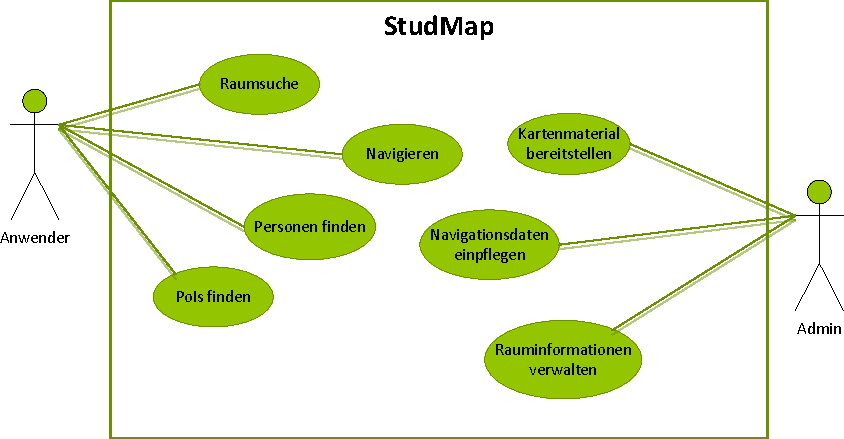
\includegraphics[width=\linewidth]{../Bilder/UseCaseDiagram}
\label{fig:UseCaseDiagram}
\end{figure}

Der Anwender hat in den meisten F�llen Interesse daran, zu besonderen
Orte, die sogenannten Points of Interest (Abk�rzung PoI), der Hochschule zu gelangen (z.B. Mensa, Dekanat). Neben diesen wird auch gelegentlich nach den verbleibenden R�umen des Geb�udes gesucht (z.B. Seminarr�ume).
F�r das Auffinden von und die Navigation zu diesen Orten wollen wir eine Anwendung entwickeln. Dar�ber hinaus sollen auf der Karte angemeldete Benutzer zu finden sein\footnote{Siehe \href{http://de.wikipedia.org/wiki/Begriffe\_der\_Harry-Potter-Romane\#Karte\_des\_Rumtreibers}{Karte des Rumtreibers}}.

Damit ein solches System funktioniert ben�tigt dies einen Administrator, der sich um das Kartenmaterial und um die Datenpflege k�mmert.

\section{Projektorganisation}
Als Plattform f�r unser Projekt verwenden wir Google Code:\\
\href{https://code.google.com/p/studmap/}{https://code.google.com/p/studmap/}

Dort nutzen wir das SVN Repository zur Quellcode Ablage und den Issue Tracker zur Verwaltung von Benutzeranforderungen und Fehlern. Wir haben uns in unserem Projekt f�r eine agile Projektorganisation nach dem Vorbild von Scrum entschieden und den Issue Tracker entsprechend konfiguriert. So stehen uns die Issue Typen User Story, Task und Bug zur Verf�gung. Zus�tzlich haben wir noch vier Kategorien eingef�hrt: ProductBacklog, SprintBacklog, OpenBugs und OpenTasks. Mittels der Kategorien k�nnen wir die verschiedenen Issues besser strukturieren.

Kurz nach Beginn des Projektes haben wir die Benutzeranforderungen in Form von User Stories\footnote{Siehe \href{https://code.google.com/p/studmap/issues/list?can=1\&q=type=UserStory\&colspec=ID\%20Type\%20Status\%20Priority\%20PartOf\%20Component\%20Owner\%20Summary}{Google Code}}
angelegt und dem ProductBacklog zugewiesen. F�r dieses Projekt haben wir uns auf Sprints mit einer Dauer von jeweils zwei Wochen geeinigt. Zu Beginn eines jeden Sprints haben wir entsprechende User Stories in den SprintBacklog �bertragen und abgearbeitet. 	% Chris	(Links auf Google Zeug und so... Projektstruktur bzw. Organisation)
\chapter{Architektur}
Die Architektur unseres Projekts sieht an der Benutzeroberfl�che neben dem Navi-gations-Client einen Collector-Client und eine Admin-Oberfl�che vor. Die Informationen in einer zentralen Datenbank gespeichert und mit Hilfe eines Webservice bereitgestellt.

\begin{figure}[H]
\centering
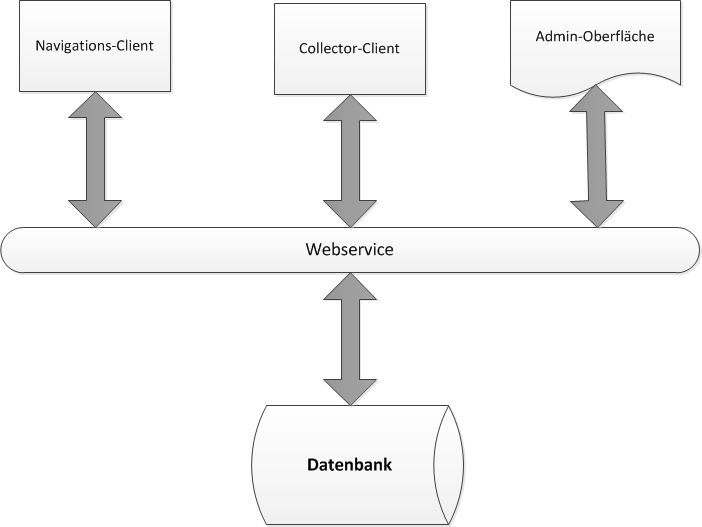
\includegraphics[width=\linewidth]{./Bilder/Architektur}
\caption{Grafische Darstellung der Architektur}
\label{fig:Achitektur}
\end{figure}

\section{Bestandteile}

Der \textbf{Navigations-Client} ist eine Anwendung f�r den Benutzers. Hier wird die Karte des Geb�udes mit allen Wegpunkten und die Navigation angezeigt. Dem Benutzer werden zus�tzlich zur Navigation Komfortfunktionen zur einfacheren und schnelleren Bedienung bereit gestellt.

Die \textbf{Admin-Oberfl�che} dient der Verwaltung von Karten und Benutzern. Der Administrator kann alte Karten bearbeiten oder neues Kartenmaterial einstellen. Zu diesen Karten wird auch der Graph mit allen Knoten und Kanten erstellt und anschlie�end verwaltet. Mit der Benutzerverwaltung k�nnen neue Benutzer angelegt und vorhandene bearbeitet werden oder aber alte Benutzerkonten gel�scht werden.

Mit dem \textbf{Collector-Client} soll der Datenbestand des Projektes fortlaufend erweitert werden. F�r die Knoten, bzw. Wegpunkte, k�nnen verschiedene, f�r die Navigation ben�tigte Informationen hinterlegt werden. Um fehlerhafte Eingaben zu vermeiden wird dieses Tool nicht vom Benutzer, sondern nur von Administratoren eingesetzt.

In der \textbf{Datenbank} werden s�mtliche Informationen der Anwendung gespeichert. Sie enth�lt die Benutzerdaten und das gesamte Kartenmaterial. Das Kartenmaterial umfasst dabei die Kartengrafiken wie auch den zugeh�rigen Graphen. �ber einen \textbf{Webservice} k�nnen die Daten abgerufen werden. Dieser stellt Funktionen zur Abfrage und Ablage von Navigations- und Benutzerdaten bereit.

Alternativ wurde uns ein Server mit einer �ffentlichen IP-Adresse an der Hochschule bereitgestellt, auf welchem das System jetzt betrieben wird.

\section{Kommunikation}
Die externen Kommunikation des Navigations-Clients, Collector-Clients und der Admin-Oberfl�che mit dem Webservice basiert auf HTTP. Als Austauschformat wird JSON verwendet.
Die interne Kommunikation des Webservices mit der Datenbank basiert auf dem Entity-Framework. 

Die westf�lische Hochschule hat einen Server mit einer festen IP-Adresse zur Verf�gung gestellt. Auf diesem betreiben wir einen IIS 7.5\footnote{\href{http://www.iis.net/}{http://www.iis.net/}} mit unserem Projekt.

	% Christoph: Ursprüngliche Idee: Windows Azure, Stand jetzt Server läuft bei uns lokal
								% Architektur Bildchen...

% Verwendung von Bibliotheken (Entity Framework, d.3 floorplan, ELMAH) im jeweiligen Kapitel
\chapter{Dom�nenmodell}
Durch das Dom�nenmodell legen wir Begriffe fest, mit denen
die Kommunikation im Projektteam vereinheitlicht und damit einfacher wird.

\section{Anwendungsstruktur}

\subsection*{Webservice (StudMap.Service)}
Stellt Funktionen zur Ablage und Abfrage von Navigationsinformationen und Benutzerdaten �ffentlich bereit.

\subsection*{Admin-Oberfl�che (StudMap.Admin)}
Weboberfl�che zum Anlegen, Bearbeiten von Navigationsinformationen und Benutzerdaten. Die Weboberfl�che kann nur von der Benutzerrolle Administrator bedient werden.

\subsection*{Navigations-Client (StudMap.Navigator)}
Eine Anwendung zur Anzeige von Karten und Navigation zwischen Wegpunkten. Diese wird durch den Anwender bedient.

\subsection*{Collector-Client (StudMap.Collector)}
Eine Anwendung zur Eingabe von Navigationsinformationen. Diese wird von Administratoren verwendet.
\section{Benutzerrollen}

\subsection*{Anwender (User)}
Der Anwender verwendet den Navigations-Client, um die k�rzeste Route zu einem gew�nschten Ziel zu erhalten.

\subsection*{Administrator}
Verwendet Admin-Oberfl�che und den Collector-Client. Dazu muss dieser registriert sein.

\section{Grundbegriffe}

\subsection*{Karte (Map)}
Beschreibt das gesamte Geb�ude mit allen Stockwerken.

\subsection*{Stockwerk (Floor)}
2-dimensionale Ansicht mit allen Layern der Ebene.

\subsection*{Schicht (Layer)}
Es gibt mehrere Schichten, die jeweils Detailinformationen zu
einem Stockwerk enthalten.

\begin{itemize}
\item Bild-Layer: Enth�lt grafische Darstellung des Stockwerks.
\item Graph-Layer: Enth�lt Kanten und Knoten f�r Routen.
\item POI-Layer: Zusatzinformationen zu speziellen Orten.
\item Routen-Layer: Darstellung grafischer Elemente zur Navigation.
\end{itemize}

\subsection*{Route}
Hat einen Start- und einen Endknoten. Verbindet diese beiden Knoten �ber Zwischenknoten und Kanten.

\subsection*{Graph}
Gesamtheit aller Knoten und Kanten der Karte (Stockwerk-�bergreifend).

\subsection*{Knoten (Node)}
Besteht aus eindeutigem Identifier, X- und Y-Koordinate und Stockwerk. Zu dem Knoten k�nnen zus�tzliche Informationen hinterlegt werden: Name, Raumnummer, NFC-Tag, QR-Tag und Verweis auf PoI.

\subsection*{Kante (Edge)}
Verbindung zweier Knoten. Bedeutet, dass man von einem Punkt zum anderen laufen kann.

\subsection*{Point of Interest (PoI)}
Ort besonderen Interesses (z.B. Bibliothek, Mensa, ...)

\chapter{Datenbank}
\label{cha:Datenbank}
Die Daten f�r StudMap werden in einer zentralen Datenbank gespeichert.
In diesem Kapitel werden die einzelnen Tabellen thematisch gruppiert
und Besonderheiten erl�utert.

\section{Kartendaten}
\label{sec:Maps}

\begin{figure}[H]
\centering
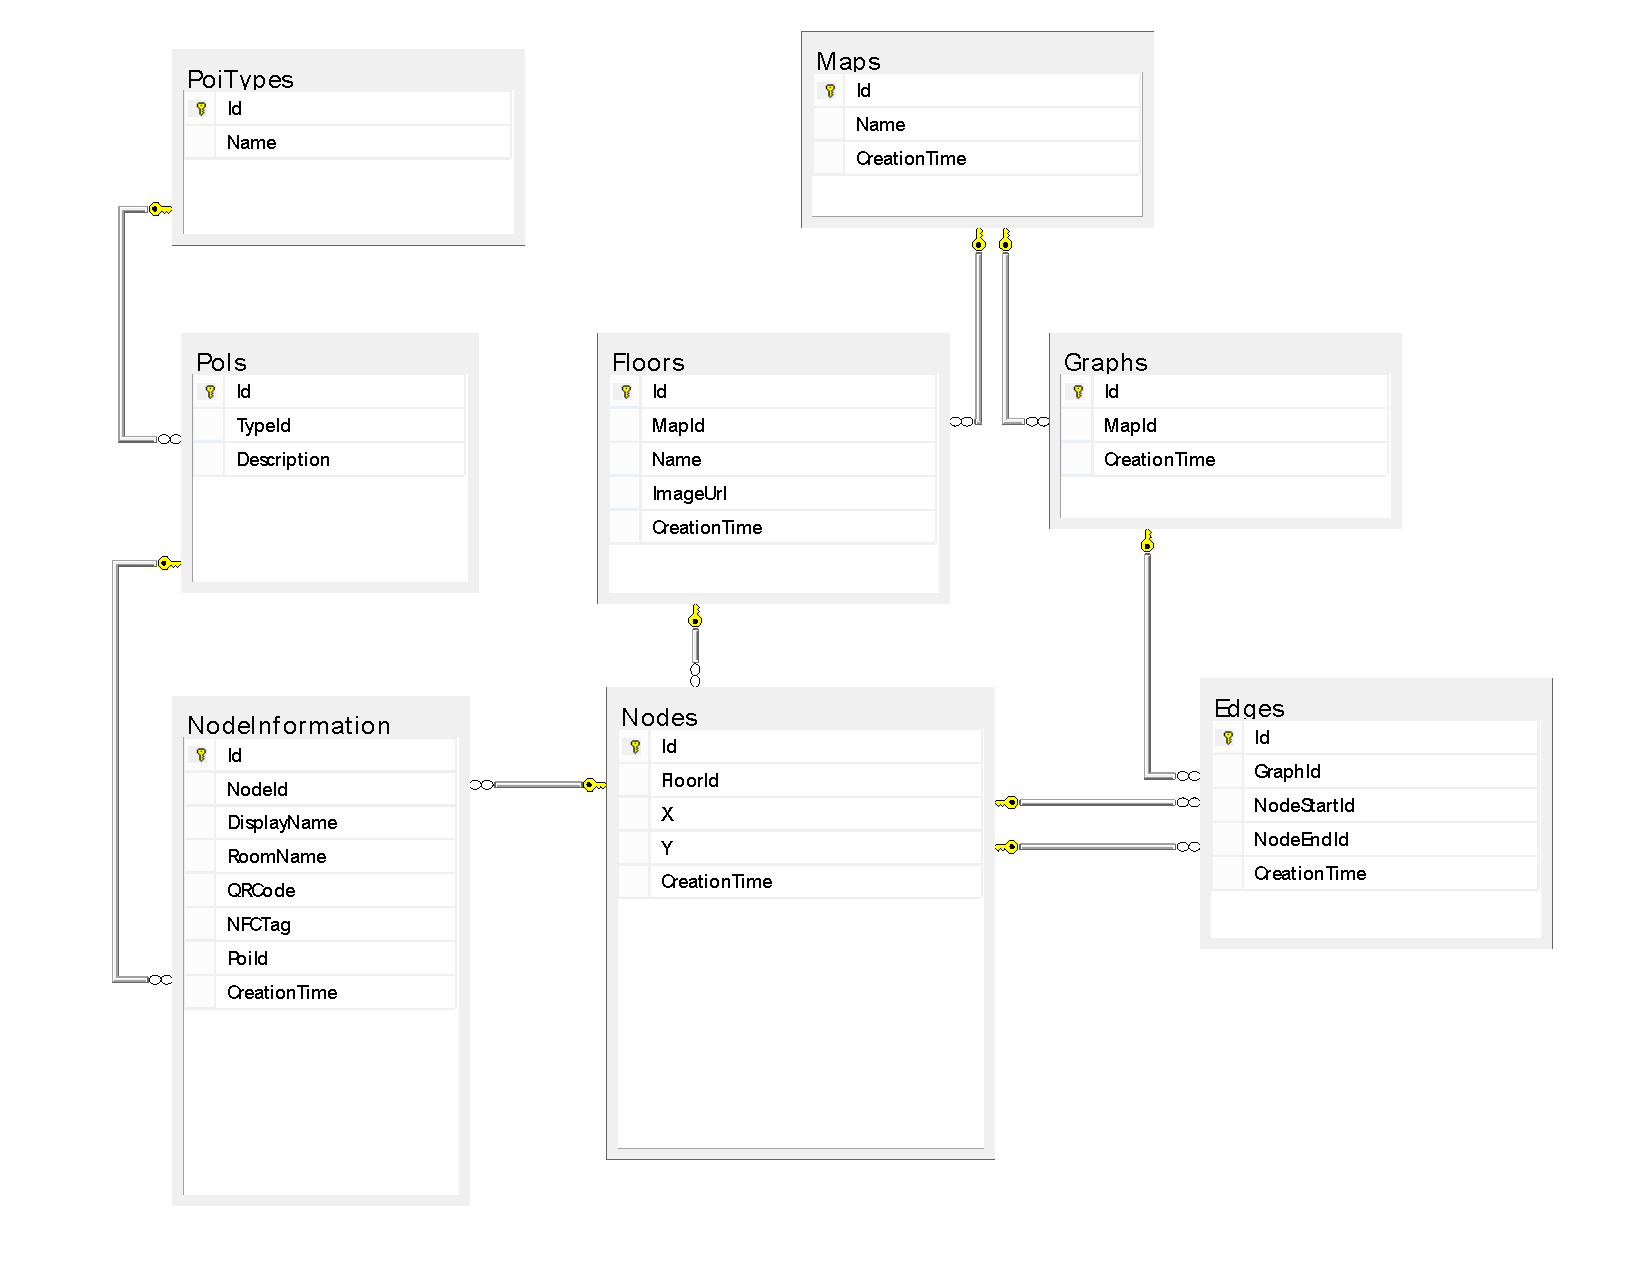
\includegraphics[width=\linewidth]{./Bilder/MapEntities}
\caption{Datenbankmodell f�r die Kartenobjekte}
\label{fig:MapEntities}
\end{figure}

\subsection{Maps}
\label{db:maps:Maps}
F�r jede Karte wird ein Eintrag in dieser Tabelle erzeugt.
Zu jeder Karte wird ein frei vergebener Name und der
Erstellungszeitpunkt gespeichert.

\begin{tabularx}{\textwidth}{|l|l|X|}
\hline \textbf{Spaltenname} & \textbf{Datentyp} & \textbf{Bedeutung}  \\ 
\hline Id 					& INTEGER (PK)		 & ID der Karte \\ 
\hline Name 				& NVARCHAR(255)		 & Name der Karte \\ 
\hline CreationTime 		& DATETIME 			 & Erstellungszeitpunkt\\ 
\hline 
\end{tabularx} 

\subsection{Floors}
F�r jedes Stockwerk wird ein Eintrag in dieser Tabelle angelegt.
Zu jedem Stockwerk wird ein frei vergebener Name, eine URL auf ein
Bild des Stockwerks und ein Erstellungszeitpunkt gespeichert.
Ein Stockwerk ist genau einer Karte zugeordnet.

\begin{tabularx}{\textwidth}{|l|l|X|}
\hline \textbf{Spaltenname} & \textbf{Datentyp} & \textbf{Bedeutung}  \\ 
\hline Id 					& INTEGER (PK)		 & ID des Stockwerks \\
\hline MapId				& INTEGER (FK)		 & ID der zugeordneten Karte \\  
\hline Name 				& NVARCHAR(255)		 & Name des Stockwerks \\ 
\hline ImageUrl				& NVARCHAR(MAX)		 & URL des Bilds \\ 
\hline CreationTime 		& DATETIME 			 & Erstellungszeitpunkt\\ 
\hline 
\end{tabularx} 

\subsection{Graphs}
Ein Graph beschreibt die Knoten- und Kantenstruktur auf einer Karte.
Dazu werden alle Kanten mit dem Graphen verkn�pft. �ber die Kanten
sind auch die Knoten mit dem Graphen indirekt verkn�pft.

\begin{tabularx}{\textwidth}{|l|l|X|}
\hline \textbf{Spaltenname} & \textbf{Datentyp} & \textbf{Bedeutung}  \\ 
\hline Id 					& INTEGER (PK)		 & ID des Graphen \\
\hline MapId				& INTEGER (FK)		 & ID der zugeordneten Karte \\  
\hline CreationTime 		& DATETIME 			 & Erstellungszeitpunkt\\ 
\hline 
\end{tabularx} 

\subsection{Edges}
Eine Kante verkn�pft zwei Knoten in einem Graphen.

\begin{tabularx}{\textwidth}{|l|l|X|}
\hline \textbf{Spaltenname} & \textbf{Datentyp} & \textbf{Bedeutung}  \\ 
\hline Id 					& INTEGER (PK)		 & ID der Kante \\
\hline GraphId				& INTEGER (FK)		 & ID der zugeordneten Graphen \\  
\hline NodeStartId			& INTEGER (FK)		 & ID des Startknotens \\  
\hline NodeEndId			& INTEGER (FK)		 & ID des Endknotens \\  
\hline CreationTime 		& DATETIME 			 & Erstellungszeitpunkt\\ 
\hline 
\end{tabularx} 

\subsection{Nodes}
Die Position eines  Knoten wird durch die Zuordnung zu einem Stockwerk
und seine X/Y-Koordinaten auf diesem Stockwerk bestimmt. Au�erdem wird
der Erstellungszeitpunkt eines Knotens gespeichert.

Die X- und Y-Koordinaten werden im Bereich 0.0 bis 1.0 gespeichert. 
Dabei bedeutet 0.0 ganz links (X) oder ganz oben (Y) und 1.0
ganz rechts (X) bzw. ganz unten (Y) auf dem Bild des Stockwerks.

\begin{tabularx}{\textwidth}{|l|l|X|}
\hline \textbf{Spaltenname} & \textbf{Datentyp} & \textbf{Bedeutung}  \\ 
\hline Id 					& INTEGER (PK)		 & ID der Knotens \\
\hline FloorId				& INTEGER (FK)		 & ID der zugeordneten Stockwerks \\  
\hline X					& DECIMAL(18,17)	 & X-Koordinate auf dem Stockwerk \\  
\hline Y					& DECIMAL(18,17)	 & Y-Koordinate auf dem Stockwerk \\  
\hline CreationTime 		& DATETIME 			 & Erstellungszeitpunkt\\ 
\hline 
\end{tabularx} 

\subsection{NodeInformation}
\label{db:maps:NodeInfo}
Zu einem Knoten k�nnen noch weitere Informationen hinterlegt werden.
Diese sind optional und werden nur zu wichtigen Knoten wie
Seminarr�umen, B�ros und Toiletten hinzugef�gt. �ber die Knoteninformationen
kann auch ein PoI mit dem Knoten verkn�pft werden.

\begin{tabularx}{\textwidth}{|l|l|X|}
\hline \textbf{Spaltenname} & \textbf{Datentyp} & \textbf{Bedeutung}  \\ 
\hline Id 					& INTEGER (PK)		 & ID der Knoteninformation \\
\hline NodeId				& INTEGER (FK)		 & ID der zugeordneten Knotens \\  
\hline DisplayName			& NVARCHAR(50)		 & Name der angezeigt werden soll \\  
\hline RoomName				& NVARCHAR(255)		 & Offizieller Raumname (z.B. B4.0.1.11) \\  
\hline QRCode				& NVARCHAR(255)		 & Hinterlegter QR-Code \\ 
\hline NFCTAG				& NVARCHAR(50)		 & Hinterlegtes NFC-Tag \\ 
\hline PoiId				& INTEGER (FK)		 & Optionaler zugeordneter PoI \\ 
\hline CreationTime 		& DATETIME 			 & Erstellungszeitpunkt\\ 
\hline 
\end{tabularx} 

\subsection{PoIs}
\label{db:maps:PoIs}
Ein PoI (Point of Interest) kategorisiert f�r den Benutzer relevante Knoten.
Hier kann z.B. nach Dozentenb�ros, Mensa, Bibliothek und Toiletten gefiltert
werden.

\begin{tabularx}{\textwidth}{|l|l|X|}
\hline \textbf{Spaltenname} & \textbf{Datentyp} & \textbf{Bedeutung}  \\ 
\hline Id 					& INTEGER (PK)		 & ID des Knotens \\
\hline TypeId				& INTEGER (FK)		 & ID des PoI-Typs \\  
\hline Description			& NVARCHAR(MAX)		 & Zus�tzliche Beschreibung des PoIs \\  
\hline 
\end{tabularx} 

\subsection{PoiTypes}
Diese Tabelle enth�lt die m�glichen Typen von PoIs.

\begin{tabularx}{\textwidth}{|l|l|X|}
\hline \textbf{Spaltenname} & \textbf{Datentyp} & \textbf{Bedeutung}  \\ 
\hline Id 					& INTEGER (PK)		 & ID des PoI-Typs \\
\hline Name					& NVARCHAR(255)		 & Name des PoI-Typs \\  
\hline 
\end{tabularx} 
\section{Users}
\label{sec:Users}

\begin{figure}[H]
\centering
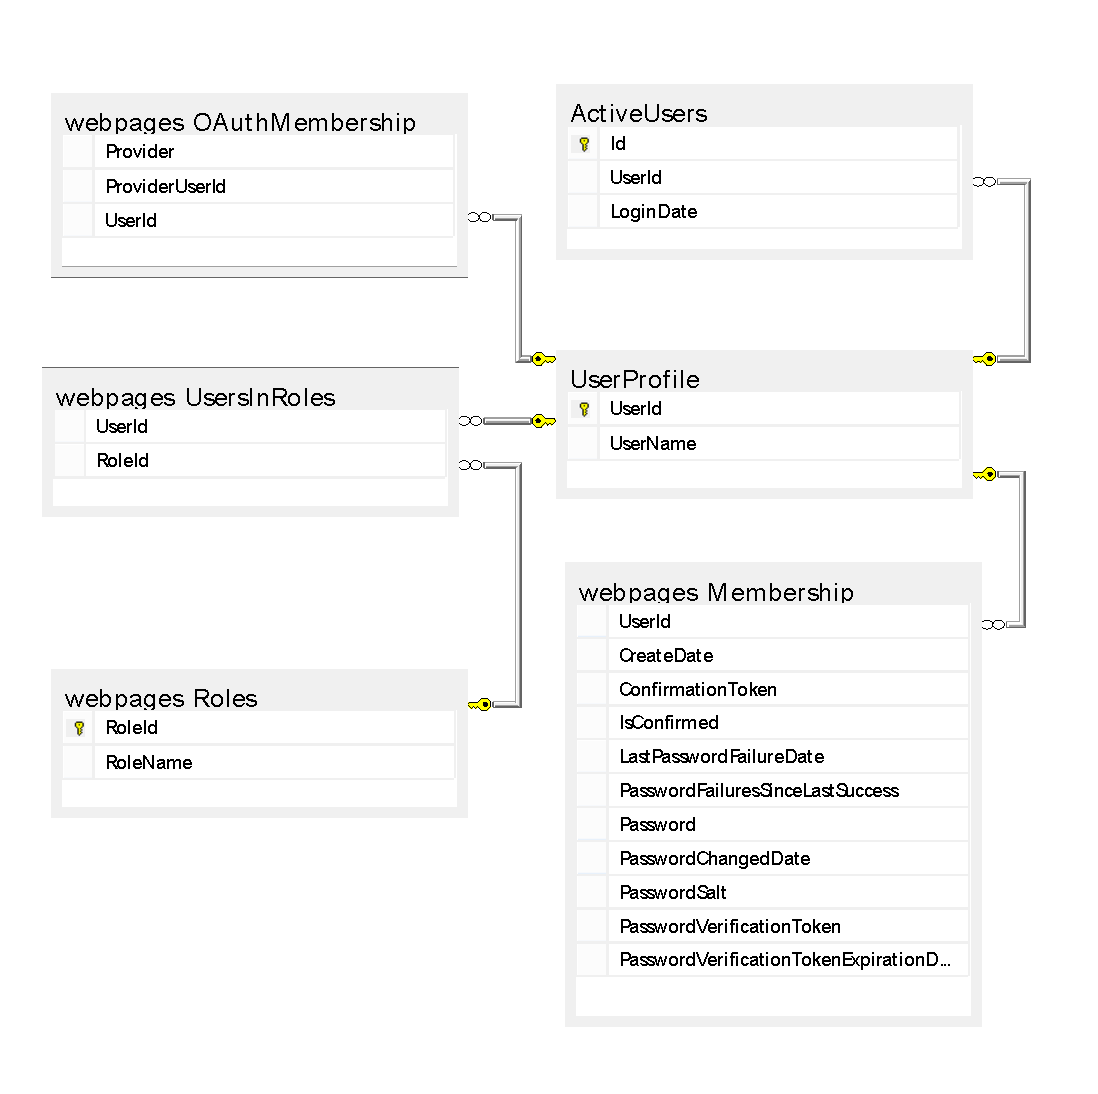
\includegraphics[width=1.0\linewidth]{./Bilder/UserEntities}
\caption{Datenbankmodell f�r Benutzerobjekte}
\label{fig:UserEntities}
\end{figure}

\subsection{MVC spezifische Tabellen}
Alle Tabellen aus dem Diagramm \ref{fig:UserEntities} mit Ausnahme der
ActiveUsers-Tabelle werden von MVC generiert und verwaltet. Sie dienen zur Benutzerauthentifizierung und zur Autorisierung. 

Relevant f�r StudMap sind die Tabellen "'webpages\_Roles"' und
"'webpages\_UserInRoles"'. Hier werden bestehenden Nutzern Rollen
zugewiesen. Um die Admin-Oberfl�che nutzen zu k�nnen, muss einem
Nutzer die Rolle "'Admin"' zugewiesen worden sein.

\subsection{ActiveUsers}
In dieser Tabelle wird festgehalten, welche Benutzer innerhalb 
eines festgelegten Zeitraums unsere App benutzt haben
Diese Tabelle kann z.B. um die letzte Position des Nutzers
erweitert werden. Dadurch k�nnten andere Nutzer sehen, wer 
gerade in ihrer N�he ist.

\begin{tabularx}{\textwidth}{|l|l|X|}
\hline \textbf{Spaltenname} & \textbf{Datentype} & \textbf{Bedeutung}  \\ 
\hline Id 					& INTEGER (PK)		 & ID des Eintrags \\ 
\hline UserId 				& INTEGER (FK)		 & ID des Nutzers \\ 
\hline LoginDate 	     	& DATETIME 			 & Zeitpunkt der letzten Anmeldung bzw. Nutzung der App\\ 
\hline 
\end{tabularx} 
		% Fabian
\chapter{Service}
Der Webservice stellt die Logik f�r alle Clients bereit. Dies schlie�t den Navigations-Client,
den Collector-Client und die Admin-Oberfl�che mit ein. Er kapselt in erster Linie die Datenbankzugriffe
und nutzt Caching f�r h�ufige Anfragen. Es werden Funktionen zur Benutzerverwaltung
sowie zur Navigation bereitgestellt.

\section{Allgemeine Struktur}
Als Grundlage verwendet der Webservice ein ASP.NET Web API
Projekt\footnote{\url{http://www.asp.net/web-api}}. Der Datenbankzugriff erfolgt
�ber das Entitiy Framework von Microsoft\footnote{ 
\url{http://msdn.microsoft.com/de-de/library/bb399567(v=vs.110).aspx}}.

In einem Web API Projekt k�nnen die Funktionen des Webservice
auf Basis von selbst definierten Datenstrukturen erstellt werden.
Damit muss sich der Entwickler nicht damit besch�ftigen, wie 
diese Objekte vom Client geliefert werden und in welchem Format
die Antwort gesendet wird. Das Serialisieren erfolgt meist
in den Formaten XML oder JSON. Unser Webservice verwendet im
Standard das JSON-Format, da es leichtgewichtiger ist und
somit besser f�r mobile Clients geeignet ist.

Die Funktionalit�t teilt sich in drei Bereiche auf. Das sind die Karten- und Navigationsinformationen, die Benutzerverwaltung
und das WLAN-Fingerprinting (nur experimentell). Diese Bereiche
werden in drei Controllern abgebildet. Ein Controller ist eine Klasse
die Anfragen gegen den Webservice verarbeitet.

\section{HTTP-Schnittstelle}
Der Webservice bietet eine HTTP-Schnittstelle, die von den Clients
genutzt wird. Diese bietet Funktionen �ber die HTTP-Methoden GET
und POST auf bestimmte URLs an.

Der Client sendet einfache Anfrageparameter �ber die URL-Query-Parameter (GET).
Bei komplexeren Anfragen kann er ein JSON-Dokument in den Body der
Anfrage setzen (POST). Als Antwort erh�lt er ein
JSON-Dokument\footnote{Web API unterst�tzt auch XML, dies wird von unseren Clients allerdings nicht verwendet}.

Eine komplette Referenz der Webservice-Funktionen befindet sich
im Anhang dieser Dokumention (siehe \nameref{cha:Webservice}).

\section{Assembly-Schnittstelle}
Da Anwendungen wie die Admin-Oberfl�che und ein Teil der Client-Oberfl�che
immer auf demselben Server laufen wie der Webservice, ist ein Umweg
�ber die HTTP-Schnittstelle aufwendiger als notwendig. Daher verwenden
diese Anwendungen auch die Assembly-Schnittstelle des Webservices.
Dabei werden die Anfragen direkt an die entsprechenden Controller
gestellt. Das Serialisieren und Deserialisieren der Anfrage- und
Antwortobjekte entf�llt somit. F�r dynmaische Anfragen, z.B. in
Javascript, nutzen diese Anwendungen allerdings weiterhin die
HTTP-Schnittstelle. 

Die Assembly-Schnittstelle bietet die gleiche Funktionalit�t wie
die HTTP-Schnittstelle. Alle Funktionen des Webservice stehen
als .NET Methoden der entsprechenden Controller-Klasse zur Verf�gung.

\section{Caching}
Der Webservice nutzt das Caching der HTTP-Laufzeitumgebung, um 
h�ufige Abfragen (z.B. allgemeine Karten- und Stockwerkinformationen)
und komplexe Berechnungen (z.B. Routen zwischen allen Knoten)
effizienter durchzuf�hren. Die Cache-Objekte sind nur f�r ein
bestimmte Dauer g�ltig (aktuell ein Stunde) und werden invalidiert,
falls sich die Stammdaten �ndern.

\section{Sicherheit}
Aus Sicherheitsgr�nden macht es Sinn die HTTP-Schnittstelle vor
der Ver�ffentlichung des Programms auf HTTPS umzustellen, da
bisher jede Kommunikation unverschl�sselt erfolgt.
		% Fabian
%Corebib
\chapter{Collector}

Der Collector ist eine Android-Applikation, die dazu dient, Daten zu vorher vom Administrator definierten Knoten/Punkten zu sammeln und 
diese entsprechend in der Datenbank zu hinterlegen. Damit ist die Applikation ein Werkzeug der Administratoren und nicht der Endbenutzer. \\
Mit der Entwicklung des Collectors haben wir eine intensive Recherche betrieben, wie wir eine Indoor-Navigation erm�glichen k�nnen.
Bevor wir das Endergebnis der Collector-Applikation n�her erl�utern, bieten wir nun einen �berblick �ber unsere Recherche-Ergebnisse.

\chapter{Recherche}
F�r die Navigation innerhalb von Geb�uden konnten wir nicht auf die g�ngigen 
Standards zur�ckgreifen, sondern mussten uns andere Wege �berlegen, wie wir 
die Nutzer innerhalb der Geb�ude lokalisieren.\\
Au�erhalb von Geb�uden ist die Lokalisierung mittels GPS sehr verbreitet und 
auch einfach und akkurat. Um eine �hnliche Lokalisierung unserer Nutzer zu 
erm�glichen haben wir uns die folgenden M�glichkeiten �berlegt.

\section{QR-Codes}
QR-Codes sind weit verbreitet, einfach zu erstellen und mit vielen Ger�ten 
einzulesen. Dadurch bieten QR-Codes die M�glichkeit Informationen einfach an 
Orten anzubringen und von Maschinen einzulesen.\\
Wir haben uns zwei Konzepte �berlegt, QR-Codes in unserem Projekt einzubauen. 
Dazu haben wir einmal die M�glichkeit betrachtet die Auswertung des QR-Codes 
am Server zu realisieren und mit der M�glichkeit verglichen die Auswertung 
direkt am Client des Nutzers zu implementieren.

\subsection{Serverseitig}
F�r die serverseitige Umsetzung hat gesprochen, dass das Smartphone keine 
Rechenleistung ben�tigt um die QR-Codes zu dekodieren. Des Weiteren wird durch 
eine serverseitige Implementierung vermieden, dass der Nutzer weitere Apps auf 
seinem Smartphone installieren muss.\\
F�r die Implementierung in den Webservice haben wir uns f�r die offene 
Bibliothek \href{http://zxingnet.codeplex.com/}{ZXing.NET} entschieden. Allerdings 
ist uns bei der Implementierung und Testen der Bibliothek direkt aufgefallen, 
dass die Bilder zuvor am Smartphone verkleinert werden m�ssen um Bandbreite zu 
sparen und die Laufzeit der Bibliothek zu verringern.Entgegen unserer Absicht wird
daf�r jedoch clientseitig Rechenleistung ben�tigt. Dar�ber 
hinaus mussten wir feststellen, dass die Bibliothek keine zuverl�ssige 
Dekodierung der QR-Codes bietet.

\subsection{Clientseitig}
Im Gegensatz zur serverseitigen Umsetzung wird bei dieser Implementierung die 
gesamte Dekodierung am Client vorgenommen. Dadurch wird die Netzlast 
verringert, der Aufwand am Client aber erh�ht.\\
Hier bot sich zum einen an eine Bibliothek in den Client aufzunehmen, oder 
eine externe Anwendung zum Dekodieren der QR-Codes zu benutzen. Wir haben uns 
schlussendlich dazu entschieden den QR-Code Reader "`Barcode Scanner"' von ZXing
zu verwenden. Dieser wird von Google empfohlen und kann zudem einfach eingebunden
werden.
\section{WLAN Fingerprinting}
Bei der Positionierung des Nutzers mittels WLAN haben wir �ber eine f�r den 
Nutzer passive Positionierung recherchiert. Alle anderen 
Positionierungsmethoden ben�tigten eine Eingabe des Nutzers. Wir haben hier 
die Eingabe der Position auf einer Karte und das Einlesen von QR-Codes oder 
NFC-Tags behandelt. Die Positionierung erm�glicht es allerdings im Hintergrund 
zu laufen und ohne Eingabe des Nutzers die Position zu bestimmen.\\
WLAN ist zur Positionierung innerhalb von Geb�uden geeignet, da es zum einen 
eine weit verbreitete Infrastruktur ist, auf vielen mobilen Plattformen 
verf�gbar ist, W�nde durchdringt und Standard WLAN Access Points bereits eine 
Lokalisierung auf Raum-Genauigkeit erm�glicht.\\
Aus all diesen Gr�nden haben wir uns mit der Positionierung mittels WLAN 
besch�ftigt. 

\subsection{Sammeln von WLAN Fingerprints}
Um sp�ter Vergleiche im Client anstellen zu k�nnen mussten wir zuerst Daten 
des Netzwerkes sammeln. Ein Access Point wird dabei eindeutig durch eine 
\textbf{BSSID} gegenzeichnet und der Client gibt Auskunft �ber die empfangene 
Signalst�rke (\textbf{RSS \footnote{RSS: received signal strength wird in dBm 
gemessen.}}), welche beobachtet und aufgezeichnet werden kann.\\
Ziel dieser Phase war es an m�glichsten vielen Punkten in der Hochschule die 
\textit{RSS} zu messen und diese zu einem Punkt auf der Karte der Hochschule 
zu speichern.\\
\missingfigure{}
Dieses Feature ist im \textit{Collector} umgesetzt.

\subsection{Kalibrierung}
Da das Sammeln der WLAN Fingerprints mit einem Smartphone realisiert wird und 
wir davon ausgehen mussten, dass nicht jeder Nutzer das gleiche Smartphone 
besitzt, mussten wir uns eine M�glichkeit der Kalibrierung �berlegen. Dazu 
haben wir �berlegt, dass der Nutzer zuerst in einer Kalibrierungsphase selbst 
einen Fingerprint erstellt von einem von uns festgelegten Ort und diesen mit 
dem von uns gemessenen Fingerprint vergleicht. Dadurch bekommen wir einen 
Faktor um den das Smartphone des Nutzer von unserem Ger�t abweicht. Da wir 
vermuten, dass die WLAN Antennen der Smartphones auch in verschiedenen 
Bereichen, hohe, mittlere und niedrige Signalst�rke, sich stark unterscheiden 
berechnen wir diesen Faktor f�r die gerade genannten Bereiche.\\
Dieser Teilbereich ist in der \textit{StudMap-App} umgesetzt.

\subsection{Positionierung mittels WLAN Fingerprints}
Um die Position eines Nutzers ermitteln zu k�nnen muss dieser, wie der 
\textit{Collector} einen Fingerprint des WLANs an seiner aktuellen Position 
erstellen. Diesen Fingerprint und seine Faktoren, welche w�hrend der 
Kalibrierung ermittelt wurden, schickt der Client zum Server, welcher durch 
Vergleiche den Standpunkt ermittelt und zur�ckgibt.\todo{Wie werden die FP 
verglichen.}\\
Dieses Feature ist auch in der \textit{StudMap-App} umgesetzt.

\section{Positionsermittlung}
In diesem Kapitel wird beschrieben, wie die Position eines Anwenders
auf der Karte bestimmt wird. Dazu werden die im Kapitel
\nameref{cha:Recherche} beschriebenen Verfahren verwendet.

\subsection{QR-Codes}
\label{QR-Tags}
An den R�umen werden QR-Codes angebracht, die eine Zuordnung 
zu einem Knoten auf der Karte erm�glicht. Hier ist zu beachten,
dass die Informationen in dem QR-Code auch von anderen Anwendungen
interpretiert werden k�nnen. Deshalb kann hier nicht nur eine Knoten-ID
hinterlegt werden.

Wir haben uns f�r folgendes JSON-Format entschieden:
\begin{lstlisting}
{
  "General": {
    "Label": "A2.1.10",
    "Name": "Aquarium"
  },
  "StudMap": {
    "NodeId": "12",
    "Url": "https://code.google.com/p/studmap/"
  }
}
\end{lstlisting}

\subsection{NFC-Tags}
\label{NFC-Tags}
Neben den QR-Codes werden auch NFC-Tags an den R�umen angebracht.
Die Knoten werden �ber die NFC-ID des Chips zugeordnet.

Um Benutzer, die den Navigations-Client nicht installiert haben, zu
informieren wird eine URL auf den NFC-Tags gespeichert. Diese
leitet auf eine Seite mit Informationen �ber den gescannten Raum
und einen Link auf unsere Projektseite. In Zukunft kann hier auch
ein Link auf den Google Play Store hinterlegt werden, um eine
einfache Installation zu erm�glichen.

Die URL sieht z.B. so aus (f�r das Aquarium):
\begin{lstlisting}
http://193.175.199.115/StudMapAdmin/Admin/NodeInfo?nodeId=847
\end{lstlisting}


\section{Allgemeine Struktur}
\label{cha:Collector}
Die Collector-Applikation wurde als Android-Applikation umgesetzt. Es wird Android 3.0 auf einem Smartphone vorausgesetzt, um alle Funktionen nutzen k�nnen.
Anhand der Recherche-Ergebnisse haben wir uns entschieden einen Positionserkennung mittels QR-Codes, NFC-Tags und Wlan-Fingerprinting zu implementieren. 
Dabei werden QR-Codes mittels eines Tools auf dem Server generiert. Es bedarf hierbei keiner weiteren Behandlung durch die Collector-Applikation. 
Dem gegen�ber stehen das Zuordnen von NFC-Tags zu Knoten und das Sammeln von Wlan-Fingerprints durch die Collector-Applikation.
Zur Erf�llung dieser beiden Aufgaben bietet die Applikation eine schlichte Benutzeroberfl�che.

\section{Benutzeroberfl�che}
\todo{Benutzeroberfl�che und Funktionsweise sind mir fremd. Thomas und Fabian, bitte erg�nzen.}

\section{Core Bibliothek}
\label{cha:Core-Bib}
Wir haben schon fr�h festgestellt, dass es eine Vielzahl an Strukturen und Funktionalit�ten geben wird, 
die sowohl in der Collector-Applikation als auch in unserer Navigator-Applikation f�r den Endbenutzer Anwendung finden.
Dem entsprechend haben wir diese in eine eigene Android-Bibliothek ausgelagert, die wir wiederum in unsere Android-Applikationen einbinden konnten.
Zu den Kernfunktionalit�ten und -Strukturen geh�ren unter Anderem folgende:
\begin{itemize}
\item Grundlegende Definitionen einer Map, eines Floors oder eines Knoten
\item Konstanten f�r die Kommunikation mit dem Webservice
\item Ein Errorhandler f�r alle grundlegenden Fehler
\item Snippets zur einfachen Kommunikation mit dem Benutzer mittels Dialogen o.�.
\item Abbildung des Webservices zur vereinfachten Nutzung
\item Javascript-Schnittstellendefinitionen f�r die Interaktion auf der Karte
\item Asynchrone Tasks f�r Webservicekommunikation inkl. entsprechender Listener
\end{itemize}
\todo{Javascript - Daniel}
%javascript Daniel
		% Dennis, Daniel, Christoph
\chapter{Admin}
Wesentlicher Bestandteil unseres Projektes war die Administrationsumgebung. Genauer musste eine Anwendung geschaffen werden, in der Navigationsdaten hinterlegt werden k�nnen. Des Weiteren muss die Administrationsanwendung Features besitzen um Routen zu definieren und Meta-Informationen zu besonderen �rtlichkeiten festhalten zu k�nnen. Die Meta-Informationen k�nnen durch Points of Interest (PoI) Daten erweitert werden.\\
Im folgenden Abschnitt wird zun�chst die allgemeine Struktur erl�utert und anschlie�end liegt das Hauptaugenmerk auf der Benutzeroberfl�che. Eine ausf�hrliche Bedienungsanleitung der Administrationsumgebung ist im Anhang unter \nameref{Admin-Doku} beigef�gt.

\section{Allgemeine Struktur}
\subsection*{ASP.NET MVC 4}
Basis unserer Projektstruktur war das 
\textit{ASP.NET MVC Framework}\footnote{\href{http://www.asp.net/mvc}{http://www.asp.net/mvc}},
welches ein Web Application Framework ist und ein Model-View-Controller-Pattern implementiert.\\
Dies erm�glichte uns, eine Webanwendung zu entwickeln, bei der die Daten (\textit{Model}) gekapselt von der Ausgabe (\textit{View}) und dem \textit{Controller} vorliegen. Die \textit{View} pr�sentiert unsere Daten und der \textit{Controller} reagiert auf Benutzereingaben und ist sozusagen das Bindeglied oder die Schnittstelle zwischen \textit{View} und \textit{Model}.

\subsection{Model}
\subsubsection*{Account}
Diese Models wurden von MVC automatisch generiert und werden bei
der Registrierung und der An- und Abmeldung von Benutzern verwendet.

\subsubsection*{Admin}
Anwendungsspezifische Daten wie Karten, Stockwerke, Knoten, usw. werden
in selbst definierten Models gekapselt.

\subsection{View}
Die Views in unserem Projekt wurden die Bereiche Account, Admin und Home unterteilt.
\subsubsection*{Account}
Enth�lt HTML-Seiten zum Registrieren, Anmelden und Verwalten des eigenen Benutzerprofils.
\subsubsection*{Admin}
Unter diese Rubrik fallen die Webseiten, mit denen der Administrator  Stockwerke und Knoteninformationen zu einer Karte hinzuf�gen kann. Dies ist die Arbeitsoberfl�che des Administrators.
\subsubsection*{Home}
Einstiegspunkt bzw. Index unserer Webseite.

\subsection{Controller}
In unserem Projekt gibt es drei Controller.

\subsubsection*{HomeController}
Der Einstiegspunkt unserer Web-Anwendung ist der sogenannte \textit{HomeController}. Dies ist der Controller, der zum Zuge kommt, sofern die anderen beiden Controller eine Interaktion oder Controller-Aufrufe mit gewissen Parametern nicht unterst�tzen.

\subsubsection*{AccountController}
Der \textit{AccountController} verarbeitet die Ereignisse, die vom Registrierungs-, LogIn- und LogOut-Verhalten eines Benutzers ausgel�st werden. Im Fokus stehen hierbei die \textbf{HTTP GET-} und \textbf{HTTP POST-Methoden}, die von der Klasse \textit{AccountController} implementiert werden.

\subsubsection*{AdminController}
Der \textit{AdminController} reagiert auf Zustands�nderungen, die beim Anlegen, Bearbeiten und L�schen von Datenmaterial in Form von Karten oder Informationen (Meta-Informationen) ausgel�st werden.\\
Relevante Funktionen sind die Methoden zum Erstellen und L�schen von Karten und Stockwerken.
Des Weiteren werden �ber diesen Controller die Routeninformationen als Graph verarbeitet und in einer Datenbank gespeichert. Detailinformationen zu einem Knoten aus einem Graphen verarbeitet dieser Controller und speichert sie ab. Diese Detailinformationen erm�glichen besondere Orte als \textit{Points of Interest} zu kennzeichnen.

\section{Benutzeroberfl�che}
Die Admin-Oberfl�che ist �ber folgenden Link erreichbar:\\
\href{http://193.175.199.115/StudMapAdmin/}{http://193.175.199.115/StudMapAdmin/}
\begin{figure}[H]
\centering
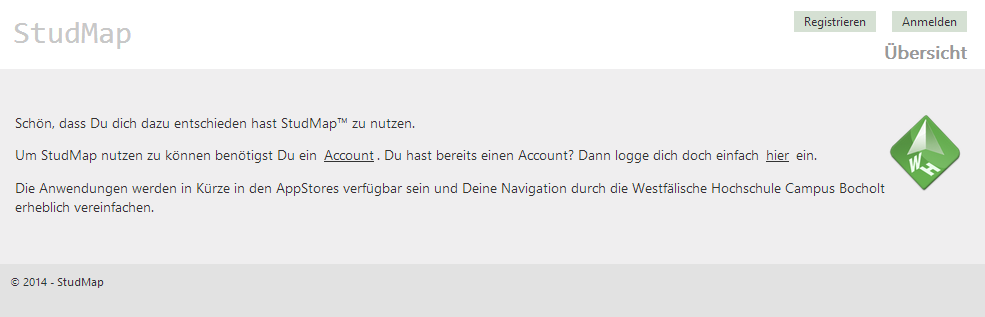
\includegraphics[width=\linewidth]{../Bilder/Admin/AdminHome}
\label{fig:AdminHome}
\end{figure}
Der Anwender hat die M�glichkeit sich anzumelden oder zu registrieren.
\subsubsection*{Registrieren}
\href{URL}{http://193.175.199.115/StudMapAdmin/Account/Register}
\begin{figure}[H]
\centering
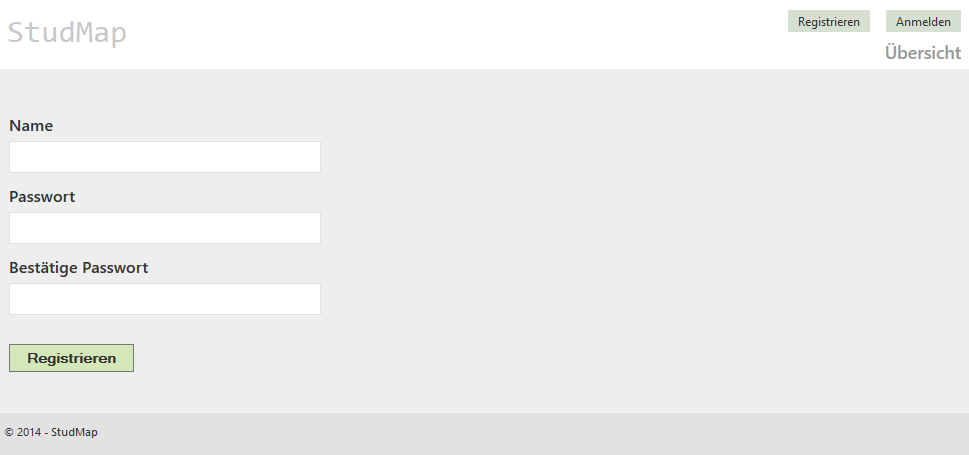
\includegraphics[width=\linewidth]{../Bilder/Admin/AdminRegistrierung}
\label{fig:AdminRegistrierung}
\end{figure}

\subsubsection*{Anmelden}
\href{http://193.175.199.115/StudMapAdmin/Account/Login}{http://193.175.199.115/StudMapAdmin/Account/Login}
\begin{figure}[H]
\centering
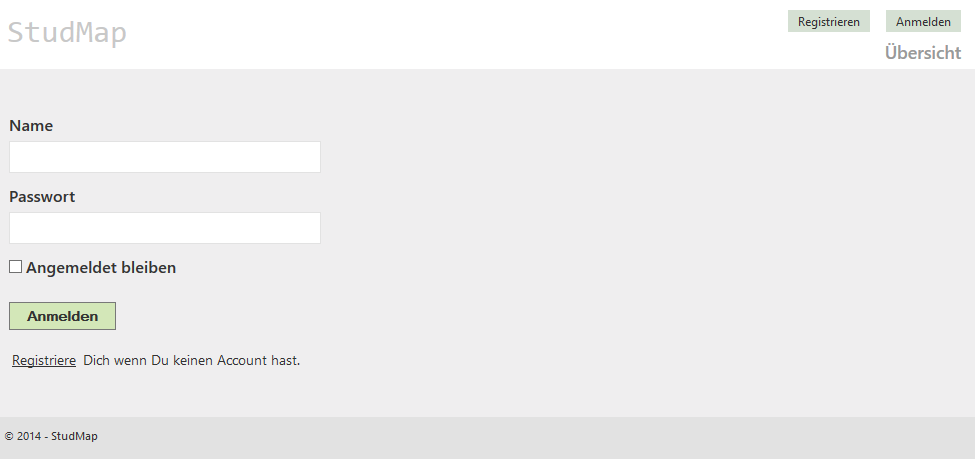
\includegraphics[width=\linewidth]{../Bilder/Admin/AdminAnmelden}
\label{fig:AdminAnmelden}
\end{figure}

\subsubsection*{Admin}
Der Einstiegspunkt zum Verwalten von Karten befindet sich unter folgendem Link: \\
\href{http://193.175.199.115/StudMapAdmin/Admin}{http://193.175.199.115/StudMapAdmin/Admin}\\
Dieser enth�lt eine Auflistung aktuell vorhandener Karten. Es  k�nnen neue Karten erstellt bzw. vorhandene entfernt werden.

\begin{figure}[H]
\centering
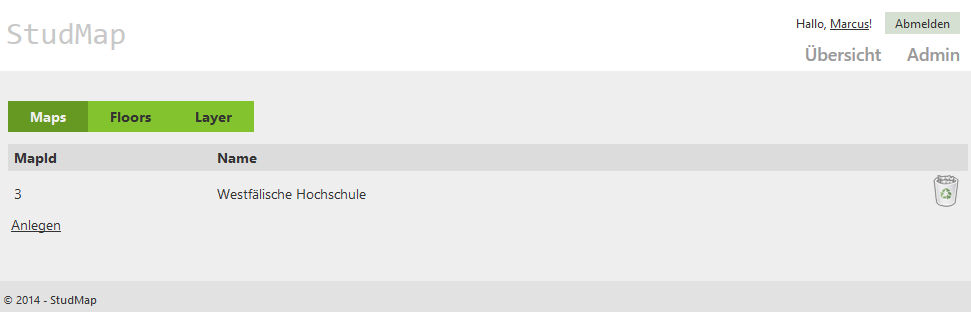
\includegraphics[width=\linewidth]{../Bilder/Admin/AdminMaps}
\label{fig:AdminMaps}
\end{figure}
Die Verwaltung der einzelnen Stockwerke zu einer Karte werden in der nachfolgenden Grafik gezeigt. Durch einen Klick auf \textit{Anlegen} kann eine neues Stockwerk mit der zugeh�rigen Kartengrundlage hinzugef�gt werden.

\begin{figure}[H]
\centering
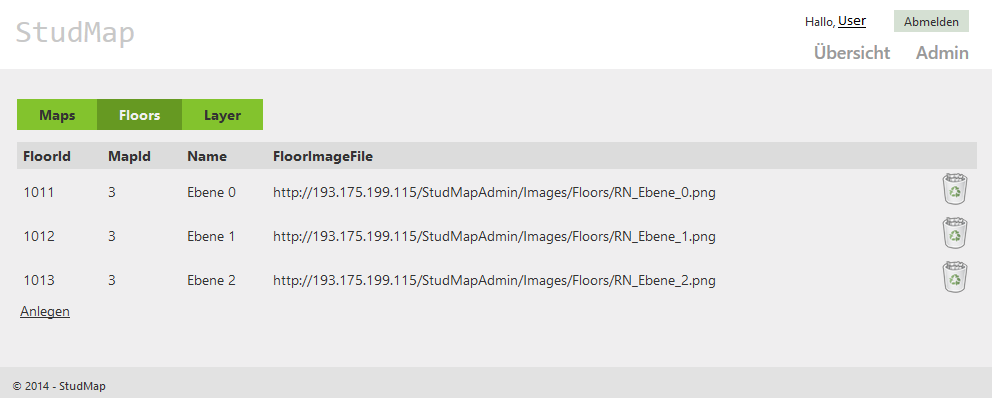
\includegraphics[width=\linewidth]{../Bilder/Admin/AdminFloors}
\label{fig:AdminFloors}
\end{figure}
Unter Layer wird die Karte und ein gegebenenfalls erstellter Graph zu genau einem Stockwerk angezeigt.
Der Administrator kann hier einen Graphen erstellen und Knoteninformationen hinterlegen. Des Weiteren besteht die M�glichkeit Knoten stockwerk�bergreifend zu verkn�pfen. Basis f�r eine ergonomische Navigation der Karte ist die JavaScript-Bibliothek \textit{D3}.

\begin{figure}[H]
\centering
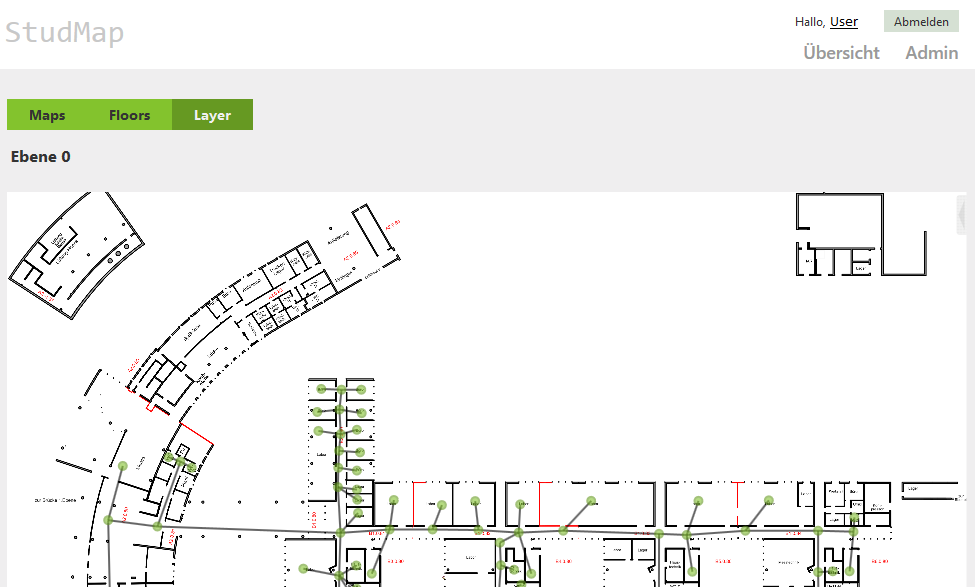
\includegraphics[width=\linewidth]{../Bilder/Admin/AdminLayer}
\label{fig:AdminLayer}
\end{figure}
\begin{figure}[H]
\centering
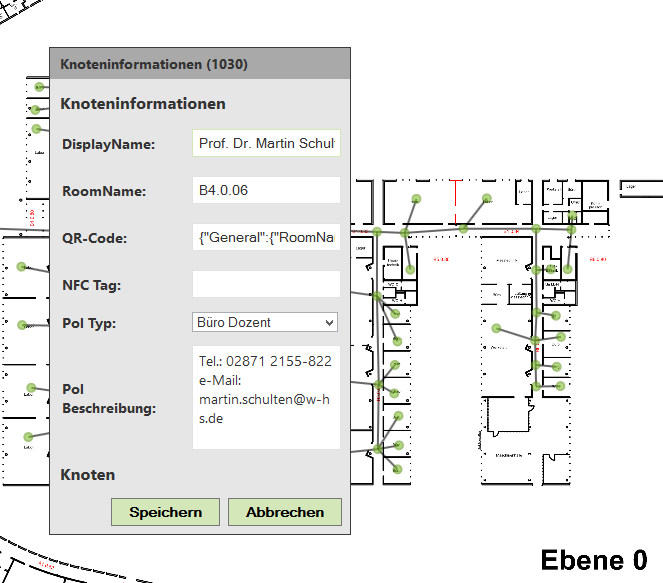
\includegraphics[width=\linewidth]{../Bilder/Admin/AdminNodeInfo}
\label{fig:AdminNodeInfo}
\end{figure}
�ber den Schaltfl�che \textit{Abmelden} gelangt man zur Hauptseite zur�ck.

\section{Admin Spezifisches}
\subsection{Neuen Benutzer mit Administrator Rechten versehen}
\label{Administrator Rechte versehen}
Nachdem ein neuer Benutzer die Registrierung erfolgreich abgeschlossen hat, ist dieser im Benutzerprofil noch nicht als Administrator gekennzeichnet. Derzeit ist es so, dass ein Datenbankadministrator in der Tabelle \textit{webpages\_UsersInRoles} den Eintrag von "`1"' f�r Users auf "`2"' f�r Admins ab�ndern muss. Nur Administratoren haben die Rechte Maps und Floors zu erstellen, sowie das Kartenmateral mit Meta-Informationen zu bereichern.

\subsection{ELMAH}
Als Logging Werkzeug haben wir das auf der .NET Plattform sehr verbreitete und OpenSource Tool \textit{ELMAH}\footnote{\href{https://code.google.com/p/elmah/}{https://code.google.com/p/elmah/}} eingesetzt. \textit{ELMAH} loggt auftretende Fehler und Exceptions.

\subsection{Maintenance Tool}
W�hrend der Entwicklung des StudMap-Projektes ist uns aufgefallen, dass 
zur Wartung und Ausf�hrung bestimmter Aufgaben ein einfaches Tool hilfreich w�re. Daher haben wir eine WPF-Anwendung entwickelt, die bisher allerdings nur QR-Codes generieren kann.

\subsubsection{QR-Codes generieren}
Eine M�glichkeit der Positionsermittlung innerhalb des StudMap-Projektes ist das 
Einlesen von QR-Codes. In diesen QR-Codes stehen die im Kapitel 
\nameref{QR-Tags} beschriebenen Daten.

In der Anwendung werden alle \nameref{object:NodeInformation} ausgelesen und 
in einer Tabelle angezeigt. Anschlie�end kann in dieser Tabelle nach 
einem \nameref{object:Floor} oder dem Namen des Raums gefiltert werden.

Abschlie�end kann f�r alle ausgew�hlten Knoten ein QR-Code als PNG generiert 
werden. Zur Generierung der QR-Codes nutzen wir die Bibliothek 
\href{http://qrcodenet.codeplex.com/}{QrCode.Net}.
			% Marcus, Chris, Fabian
\chapter{Client}
Der Client ist eine Android-Applikation f�r den Endbenutzer. Es handelt sich hierbei um einen Navigator. 
Wie jedes handels�bliche Navigationsger�t beinhaltet auch unsere Applikation eine Karte, in unserem Fall ein Geb�udeplan, 
da wir uns in unserem Projekt mit Indoor-Navigation besch�ftigen. Dar�ber hinaus kann man einen Zielpunkt w�hlen
und mit Hilfe eines QR-Codes, NFC-Tags oder des Wlans seine Position bestimmen. Sind Start und Zielpunkt bekannt, berechnet der Server
eine Route und teilt diese dem Client mit, welcher diese daraufhin graphisch auf der Karte zur Anzeige bringt. \\
Des Weiteren gibt es Suchfunktionen und Auflistungen von besonders interessanten Orten (Points of Interest).
Zur Benutzung der Wlan-Positionserkennung ist eine Registrierung und Anmeldung an unserem Server von N�ten.

\section{Allgemeine Struktur}
Die Navigator-Applikation wurde wie auch der Collector in Android umgesetzt. Es wird mindestens die Version 4.1 vorausgesetzt.
Es galt folgende Hauptaufgaben zu erf�llen:

\subsection{Positionserkennung}
Wie bereits im Kapitel \nameref{cha:Collector} beschrieben, haben wir uns f�r 
Positionserkennung anhand von QR-Codes, NFC-Tags und Wlan-Fingerprinting 
entschieden.
F�r die Positionserkennung mittels NFC und WLAN greifen wir auf unsere 
Android-Bibliothek der Kernfunktionalit�ten zur�ck. W�hrend f�r die 
Interpretation des QR-Codes
eine Fremd-Applikation zum Einsatz kommt. Diese muss bei der ersten Benutzung gegebenenfalls installiert werden. \\
Die letztendlich ermittelten Daten interpretieren wir mit Hilfe des Webservices, der wiederum Bestandteil unserer Kernfunktionalit�ten ist.

\subsection{Anzeige und Navigation auf einer Karte}
Wir haben uns f�r die Benutzung einer freien Bibliothek zur Anzeige von Karten 
entschieden. Nach intensiver Recherche fiel unsere Wahl dabei auf die 
Javascript Bibliothek \href{http://dciarletta.github.io/d3-floorplan/}{Floor 
Plan}. Diese Bibliothek setzt auf der bekannten Javascript Bibliothek 
\href{http://d3js.org/}{D3.js} auf, die Daten in HTML Dokumenten visualisiert.


Das hat zur Folge, dass unsere Karte lediglich in einer Website platziert ist, die mittels eine WebView zur Anzeige gebracht wird. Dies hat f�r uns und den Endbenutzer
den gro�en Vorteil, dass �nderung an der Karte nicht ein Update der Applikation nach sich zieht.
Mittels einer definierten Schnittstelle l�sst sich das Javascript aus unserer Android-Applikation heraus bedienen, so dass beispielsweise Positionsermittlungen automatisch 
auf der Karte nachgehalten werden. Dadurch ist die Navigation bei gew�hlten Zielpunkt vollst�ndig.

\subsection{Visuell ansprechende und intuitiv bedienbare Applikation}
Eine Applikation sollte heute intuitiv bedienbar, �bersichtlich und ansprechend sein, damit sie gerne und viel benutzt wird. Wir bauen dabei auf moderne M�glichkeiten des
Android Betriebssystems. Im folgenden Kapitel werden wir diese n�her erl�utern.

\section{Benutzeroberfl�che}
Neben der bereits erw�hnte WebView mit einer h�bschen Karte auf Basis der d3 
Bibliothek, ist unsere gesamte Applikation in dunklen T�nen gehalten und 
bietet klare Linien bei
einer Highlight-Farbe die dem Gr�n der Westf�lischen Hochschule sehr nahe kommt. 
Im Vordergrund der Applikation steht selbstverst�ndlich die Karte, w�hrend grundlegende Funktionen wie die Suche oder der Aufruf des QR-Code-Scanners in der Actionbar geboten werden.
Weitergreifende Funktionalit�ten wie das Wechseln der Ebene oder Anmelden befinden sich in einem Drawer auf der linken Seite der Applikation, der auf Wunsch in das Bild hinein gezogen
werden kann. \\
Zus�tzliche Fenster wie z.B. die Auflistung der Points of Interest werden 
grunds�tzlich in Dialogfenstern zur Anzeige gebracht, was der 
�bersichtlichkeit und Navigation durch die Applikation zu Gute kommt. Die 
Suche ist ein besonderes Event, welches in der Actionbar ausgef�hrt wird und 
dort die Anzeige ver�ndert, sodass grunds�tzlich Ordnung in der Applikation 
herrscht.
Neben dem intuitiv Design der Applikation ist selbstverst�ndlich auch die Bedienung der Karte �u�erst benutzerfreundlich. Neben den bekannten M�glichkeiten des Multitouch, beispielsweise zum Zoomen, ist auch die Steuerung der Navigation selbsterkl�rend. Einen gew�nschten Punkt angeklickt, schon kann es los gehen. Optisch ansprechend wird eine Route eingezeichnet und mit der Zielflagge gekennzeichnet.


% TODOS:
% - Funktionsweise
% - UI Aspekte
% - Android Zeug...
% - Verweis auf Anhang f�r Bedienungsanleitung / Installationsanleitung			% Dennis, Daniel, Christoph

\chapter{Fazit}

%\section{Lokalisierung innerhalb von Geb�uden}
Im Verlauf unseres Projektes ist deutlich geworden, dass die Navigation und die Lokalisierung innerhalb von Geb�uden ein schwieriges Thema ist. Daher w�hlten wir f�r das Problem der Lokalisierung gleich mehrere Ans�tze. Jedoch mussten wir erkennen, dass sowohl die Positionierung mittels Texterkennung der Raumschilder, als auch die Positionsermittlung �ber WLAN Finger Prints f�r unsere Anforderungen nicht bzw. nicht gut genug funktioniert haben.
Aus diesem Grund besch�ftigten wir uns mit alternativen M�glichkeiten und entschieden uns daf�r die Positionsdaten auf NFC Tags und QR Codes zu speichern und diese im Geb�ude zu platzieren. So ist die zuverl�ssige Positionsbestimmung immer durch Scannen eines NFC Tags oder eines QR Codes m�glich.

%\section{Verwendete Technologien}
Bei der Umsetzung dieser Ideen haben wir uns f�r ein Backend basierend auf Microsoft Technologien entschieden. F�r die Entwicklung der Datenbankstruktur verwendeten wir das Entity Framework, mit dem die Datenbank automatisch aus unserem Datenmodell generiert werden konnte. Zus�tzlich konnten komplexe Datenbankabfragen einfach umgesetzt und ausgewertet werden. Dadurch haben wir gerade zu Beginn des Projektes eine Menge Arbeit und Zeit gespart. Des Weiteren haben wir uns bei der administrativen Oberfl�che f�r eine ASP.NET Webapplikation entschieden, in der wesentliche Bestandteile der Benutzeroberfl�che und eine Benutzerverwaltung bereits integriert waren. Auch dadurch haben wir uns viel Arbeit erspart und konnten uns auf die Wesentlichen Probleme konzentrieren.

%\subsection{Zusammenarbeit mit Microsoft}
Begeistert von diesen vielen M�glichkeiten entschieden wir uns unsere Anwendung in der Windows Azure Cloud zu hosten und meldeten daher einen entsprechenden Studenten Account bei Microsoft an. Leider erhielten wir �ber Wochen kein eindeutiges Feedback von Microsoft weshalb wir uns letztendlich f�r einen eigenen Windows Server innerhalb der Hochschule entschieden haben.

%Im Frontend haben wir uns f�r eine Android Anwendung entschieden, bei der wir die wesentlichen Bestandteile in Form von Webseiten abgebildet haben. Das f�hrte %zu einer hohen Wiederverwendbarkeit, da die Anzeige der Karte in allen Anwendung benutzt wurde.

%\section{Projektmanagement}
Abschlie�end blicken wir auf ein komplexes Projekt mit vielen Herausforderungen zur�ck. Durch die unterschiedlichen Technologien haben wir alle etwas Neues kennengelernt und weitere wichtige Erfahrung sammeln k�nnen. Innerhalb des Projekts gab es allerdings nicht nur technische Herausforderungen, auch die Projektorganisation selbst, sowie die Zusammenarbeit im Team ist in jedem Projekt eine Herausforderung. Gemeinsam haben wir es, trotz der vielen Schwierigkeiten, geschafft unser Projektziel zu erreichen. So sind insgesamt drei Anwendungen zur Navigation innerhalb unserer Hochschule entstanden, die mit entsprechenden administrativen Aufwand auch wirklich eingesetzt werden k�nnten.			% Chris
%Erweiterung der Navigation.. flie�ende Navigation mit Richtungsangaben, Distanzangaben, Sprachausgabe
%Verkn�pfung mit weiteren Informationen wie Stundenpl�nen, Sprechstundenzeiten usw.
%Ausweitung auf andere Locations
%Positionsermittlung von Freunden und Navigation zu diesen
%Anbindung von Social Networks
%Sticky Notes in virtuellen R�umen


\chapter {Ausblick}
Nach Abschluss unserer Projektarbeit bleiben noch viele innovative Ideen offen. Dazu geh�ren Dinge, die in handels�blichen Navigationsger�ten zum Standard geh�ren genauso wie kreative Ideen, die das heutige Internetzeitalter erm�glicht.

Entsprechend der Erwartung eines Benutzers, sollte eine Navigation flie�end stattfinden, das hei�t anhand der aktuellen Position werden richtungsweisende Pfeile eingeblendet, eine Sprachausgabe unterst�tzt die Wegfindung und eine Angabe �ber die noch zu gehende Distanz informiert den Benutzer. Diese und �hnliche Funktionen kennt man bereits aus handels�blichen Navigationsger�ten und k�nnte sich eben bei diesen Denkanst��e f�r Erweiterungen einholen.

Grunds�tzlich besteht die M�glichkeit unser System auch in anderen Geb�uden, wie Universit�ten oder �ffentlichen Einrichtungen, einzusetzen. Es erfordert lediglich eine entsprechende Administration und Einrichtung des Systems.

Des Weiteren bietet es sich an die in einem Knoten gespeicherten Informationen deutlich zu erweitern. Da g�be es zum einen die Idee Stundenpl�ne oder Sprechstundenzeiten mit den Knoten zu verkn�pfen oder zumindest auf externe Anwendungen, die den gew�nschten Zweck erf�llen, zu verlinken. Zum anderen k�nnte man eine virtuelle Pinnwand den Knoten zu weisen, auf denen jegliche Art von �ffentlich oder auch privaten Nachrichten hinterlassen werden k�nnen. Private Nachrichten lie�en sich erm�glichen, wenn man eine Art Freundesliste pflegt. Die bereits registrierten Mitglieder bieten dazu eine gute Grundlage.
Dar�ber hinaus w�rde eine solche Freundesliste den Weg ebnen, den Aufenthaltsort von Freunden in dem Geb�ude sehen und sich dorthin navigieren lassen zu k�nnen.

Die bereits vorgestellten Erweiterungsm�glichkeiten sind selbstredend nicht alle vorstellbaren.
Der Fantasie und dem Erfindergeist der Entwickler sind keine Grenzen
gesetzt mit Ausnahme derer, dass die Anwendung benutzbar und benutzerfreundlich
bleiben sollte.

Um eine letzte Vision mit auf den Weg zu geben, w�re dem Benutzer vielleicht daran
gelegen Informationen in sozialen Netzwerken teilen zu k�nnen. Eine M�glichkeit dies mittels eines einfachen Knopfdruckes zu erledigen, ist eine von vielen verbleibenden Komfortm�glichkeiten.		% Chris & Dennis

\appendix
\chapter{Server}
Der Webserver ist unter 193.175.199.115 erreichbar:

\begin{itemize}
\item StudMap.Admin: \href{http://193.175.199.115/StudMapAdmin}{http://193.175.199.115/StudMapAdmin}
\item StudMap.Client: \href{http://193.175.199.115/StudMapClient}{http://193.175.199.115/StudMapClient}
\item StudMap.Service: \href{http://193.175.199.115/StudMapService}{http://193.175.199.115/StudMapService}
\end{itemize}


\section{Software}
Auf dem Server sind folgende Softwarekomponenten installiert:
\begin{itemize}
\item Internet Information Services (Version 7.5)
\item Microsoft SQL Server 2012
\end{itemize}

\section{Einrichtung IIS}

\begin{wrapfigure}{r}{0.4\textwidth}
\vspace{-20pt}
  \begin{center}
    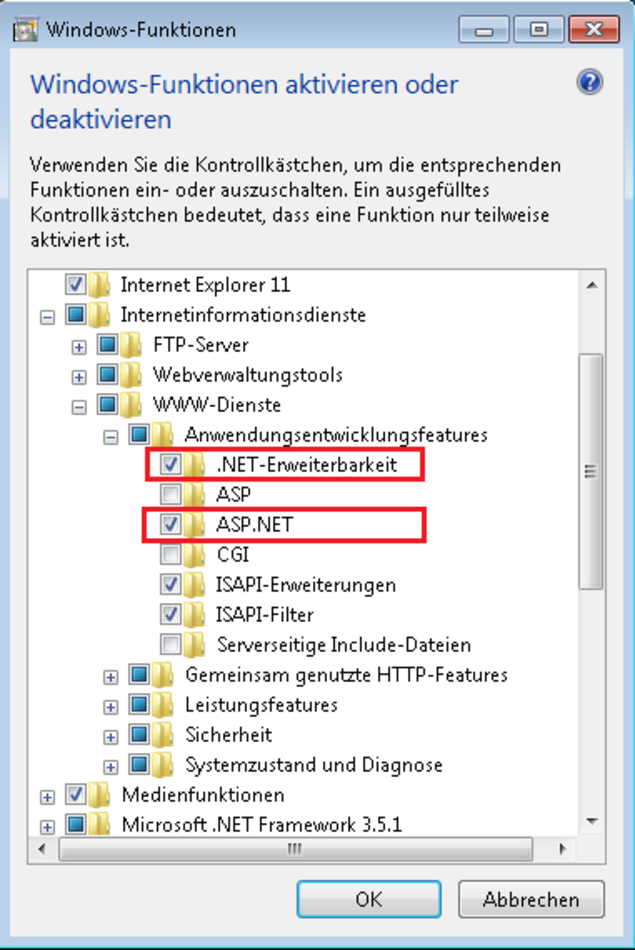
\includegraphics[width=0.9\linewidth]{../Bilder/Install_IIS}
  \end{center}
  \vspace{-20pt}
\end{wrapfigure}

Der IIS kann sowohl auf einem Windows Server als auch auf einer normalen Windows Installation eingerichtet werden. Dazu w�hlt man unter "`Programme"' > "`Windows-Features installieren oder deinstallieren"' aus. Daraufhin �ffnet sich ein Dialog (s. Abbildung), indem der IIS zur Installation ausgew�hlt werden kann.

Nach Abschluss der Installation steht der IIS-Manager zur Verf�gung und Webseiten k�nnen eingerichtet werden. 

Da auf unserem Server kein Serverbetriebssystem, sondern lediglich ein Standard Windows 
installiert ist, steht "`Web Deploy"' nicht zur Verf�gung. Daher m�ssen Deployment Pakete
manuell erstellt und auf dem Server aufgespielt werden. Dazu klickt man in Visual Studio 
auf den Kontextmen�punkt "`Ver�ffentlichen"' des jeweiligen Projektes. Anschlie�end kann
das Deployment Package im IIS �ber einen Rechtsklick auf "`StudMap"'>"'Bereitstellen"'>"'Anwendung importieren"' 
importiert werden.

\section{Einrichtung SQL Server}
Im Projekt wird ein Microsoft SQL Server 2012 verwendet. Da unsere Anwendung 
auf komplexe Managementfunktionen verzichtet kann auch die kostenlose Express 
Version genutzt werden.

Der Aufbau der Datenbank kann aus dem im SVN eingecheckten  
\href{https://studmap.googlecode.com/svn/database/StudMapDBSkript.sql}{Datenbankskripten} hergestellt werden.

\chapter{Benutzerverwaltung}
\label{Benutzerverwaltung}
In einem ASP.NET MVC 4 Projekt ist bereits eine vollst�ndige Benutzerverwaltung integriert,
die wir auch in unserem Projekt benutzen wollen. Durch die integrierte Benutzerverwaltung 
sind Webseiten zur Registrierung und f�r den Login / Logout bereits fertig. 

\begin{figure}[H]
\centering
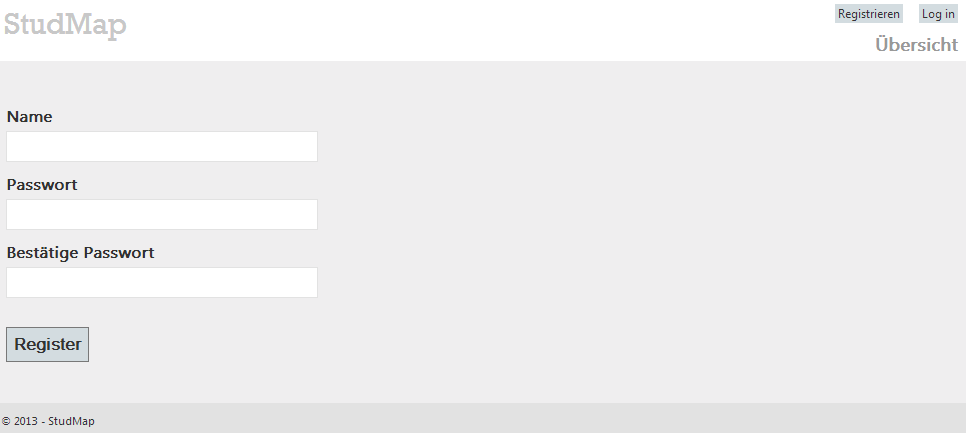
\includegraphics[width=0.7\linewidth]{../Bilder/RegisterSite}
\caption{Webseite zur Registrierung im StudMap Admin}
\label{fig:RegisterSite}
\end{figure}

F�r die Benutzerverwaltung verwendet das ASP.NET MVC 4 Projekt folgende Datenbankstruktur:
\begin{figure}[H]
\centering
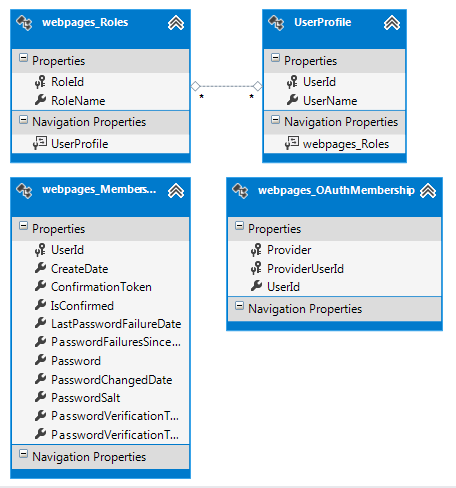
\includegraphics[width=0.7\linewidth]{../Bilder/GeneratedUserEntities}
\caption{Datenbankstruktur der integrierten Benutzerverwaltung}
\label{fig:GeneratedUserEntities}
\end{figure}

F�r unser Projekt sind nur die drei Tabellen \texttt{UserProfile}, \texttt{webpages\_Roles} und \texttt{webpages\_Membership} relevant. Wie im Domain Model bereits beschrieben unterscheiden wir zwischen den Benutzerrollen Benutzer und Administrator. Jeder Anwender kann sich in mehreren Benutzerrollen befinden. Zus�tzlich sind in der Tabelle \texttt{webpages\_membership} weitere Anwenderdaten wie beispielsweise das Datum der Registrierung das Passwort hinterlegt. Damit ist die Benutzerverwaltung f�r den Administrationsbereich vollst�ndig.


Um die (beispielsweise �ber das Smartphone) am System angemeldeten Clients zu verwalten haben wir eine weitere Tabelle \texttt{ActiveUsers} hinzugef�gt:

\begin{figure}[H]
\centering
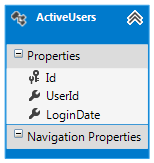
\includegraphics[width=0.7\linewidth]{../Bilder/ActiveUsersEntity}
\caption{Tabelle ActiveUsers}
\label{fig:ActiveUsersEntity}
\end{figure}


F�r den StudMap Admin gen�gt die bereits integrierte Benutzerverwaltung. Allerdings ben�tigen wir noch eine Schnittstelle, damit auch die Web bzw. Smartphone Clients auf die Benutzerverwaltung zugreifen k�nnen.
Siehe dazu Kapitel \ref{Webservice_UsersController}

\section{Collector}
\label{appendix:collector}
\subsection{Startbildschirm}
Nach Start der Anwendung befindet man sich auf dem Startbildschirm:
\begin{figure}[H]
\centering
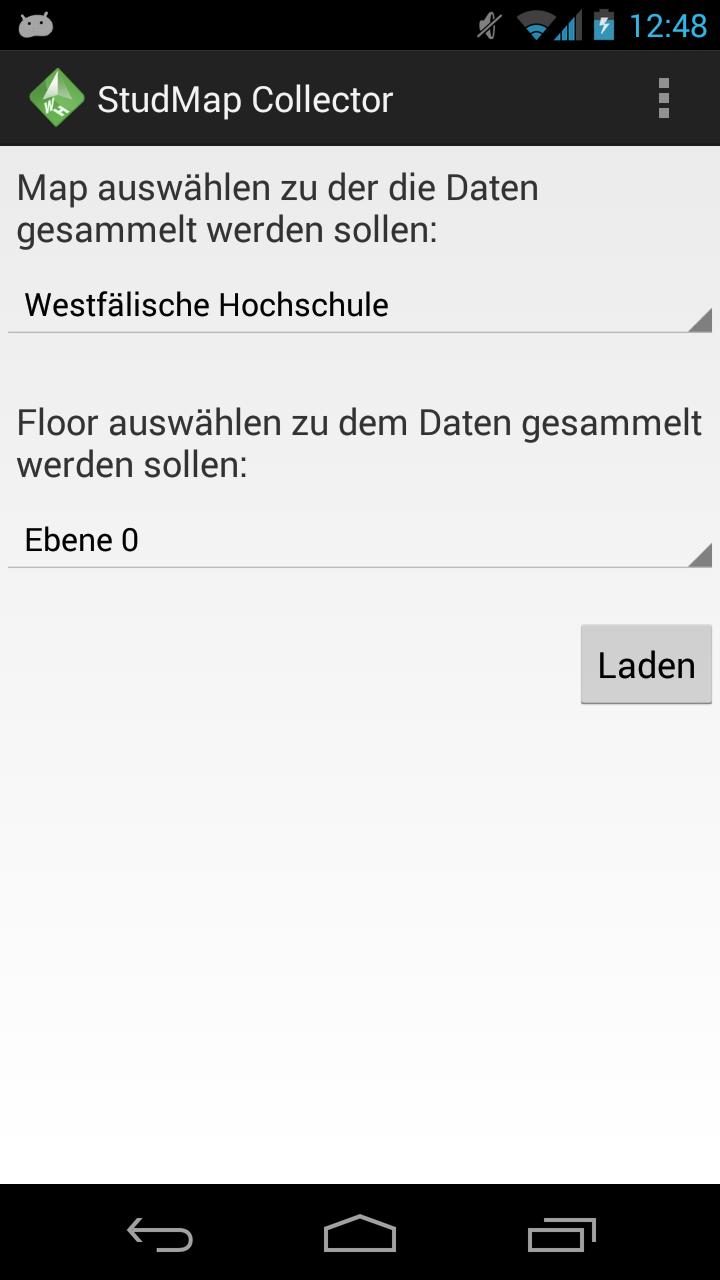
\includegraphics[width=0.5\linewidth]{../Bilder/Collector/StartScreen}
\label{fig:StartScreen}
\end{figure}
Hier k�nnen Karte und Stockwerk f�r die Datenerfassung ausgew�hlt werden. �ber den Button Laden wird die entsprechende Auswahl geladen.

\newpage

\subsection{Stockwerkansicht}
Hier sieht man das ausgew�hlte Stockwerk mit den zur Verf�gung stehenden Datenpunkten, die gr�n dargestellt sind.
\begin{figure}[H]
\centering
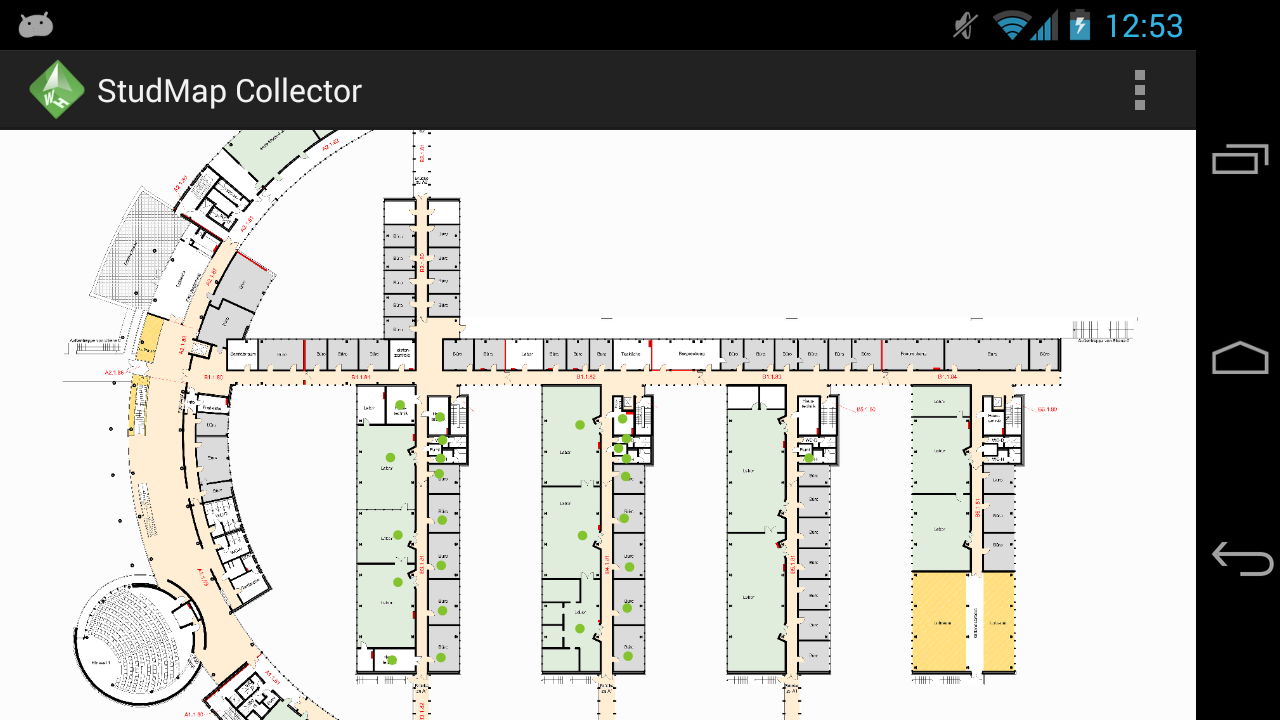
\includegraphics[width=0.8\linewidth]{../Bilder/Collector/FloorScreen}
\label{fig:FloorScreen}
\end{figure}

\subsubsection{Datenpunktauswahl}
Bei der Auswahl eines Datenpunktes erscheint folgender Dialog:
\begin{figure}[H]
\centering
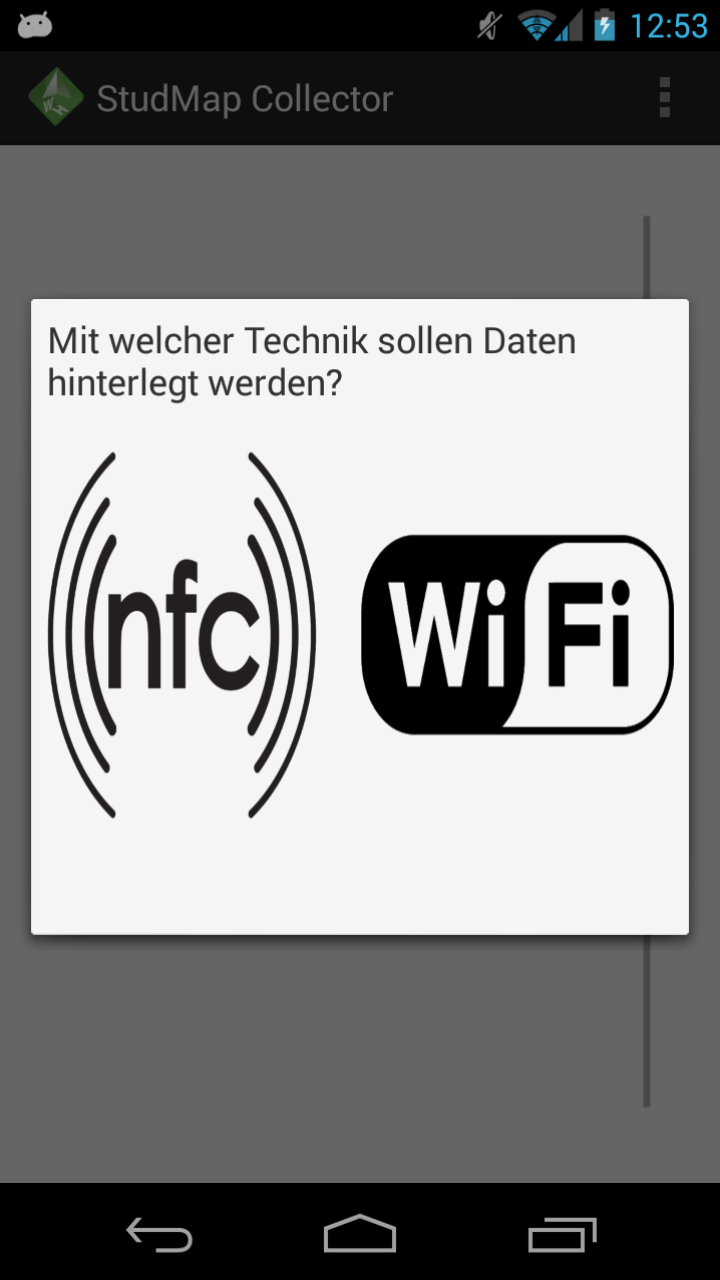
\includegraphics[width=0.35\linewidth]{../Bilder/Collector/StoreDataScreen}
\label{fig:StoreDataScreen}
\end{figure}
�ber diesen Dialog k�nnen f�r den ausgew�hlten Datenpunkt Positionsdaten hinterlegt werden. Dazu stehen die beiden Techniken NFC und Wifi zur Verf�gung.

\paragraph{NFC-Tag Ansicht}
Solange das Ger�t keinen Kontakt zu einem NFC Tag hat, wird nur die ID des Datenpunkts ausgegeben.
\begin{figure}[H]
\centering
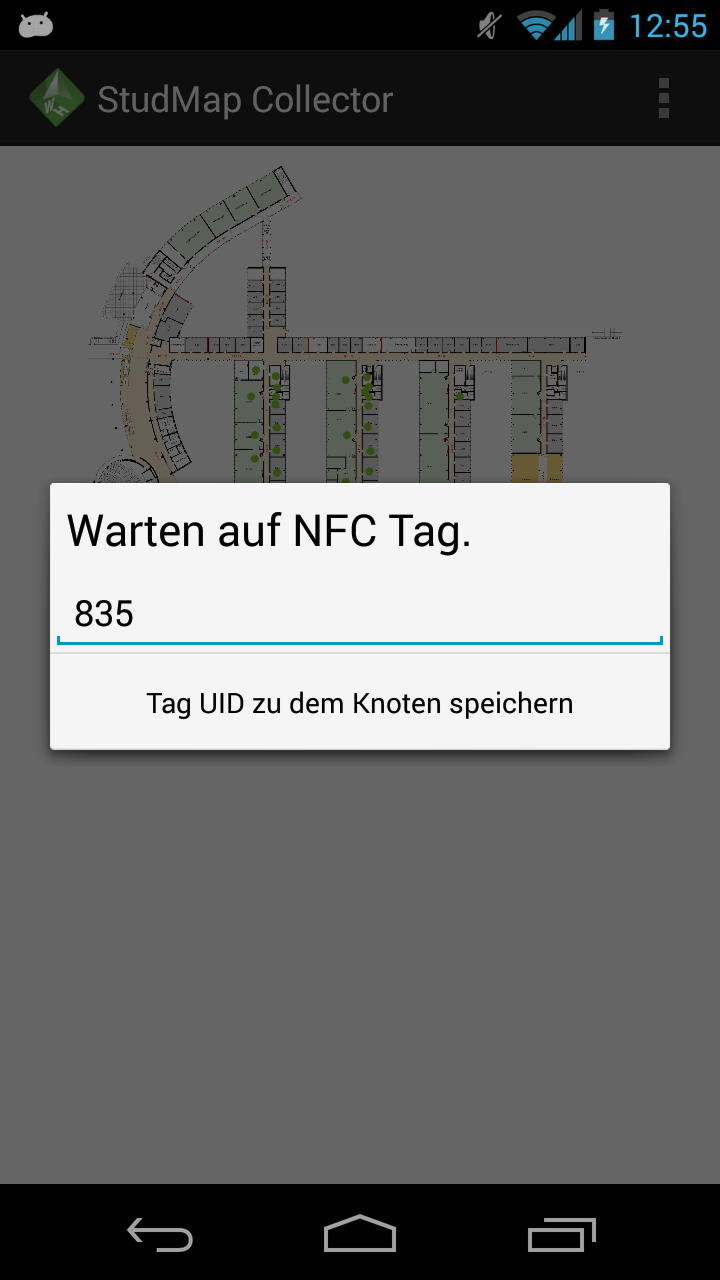
\includegraphics[width=0.35\linewidth]{../Bilder/Collector/NfcScreen}
\label{fig:NfcScreen}
\end{figure}

Sobald ein NFC Tag gefunden wurde, wird auch die ID des NFC-Tags im Dialog angezeigt und der Datenpunkt kann mit dem NFC-Tag verkn�pft werden.
\begin{figure}[H]
\centering
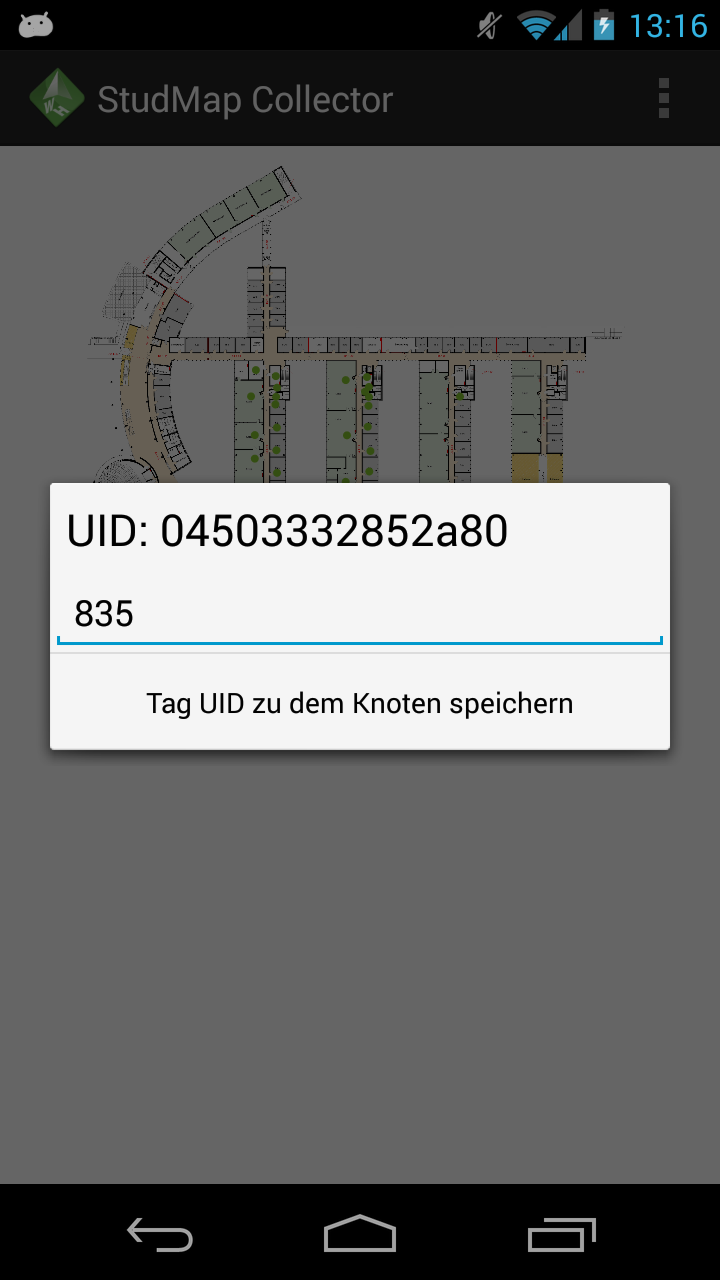
\includegraphics[width=0.35\linewidth]{../Bilder/Collector/NfcScreenRead}
\label{fig:NfcScreenRead}
\end{figure}

\newpage

\paragraph{Wifi}
�ber diesen Dialog kann f�r den ausgew�hlten Datenpunkt ein WLAN-Fingerprint erstellt und gespeichert werden.
\begin{figure}[H]
\centering
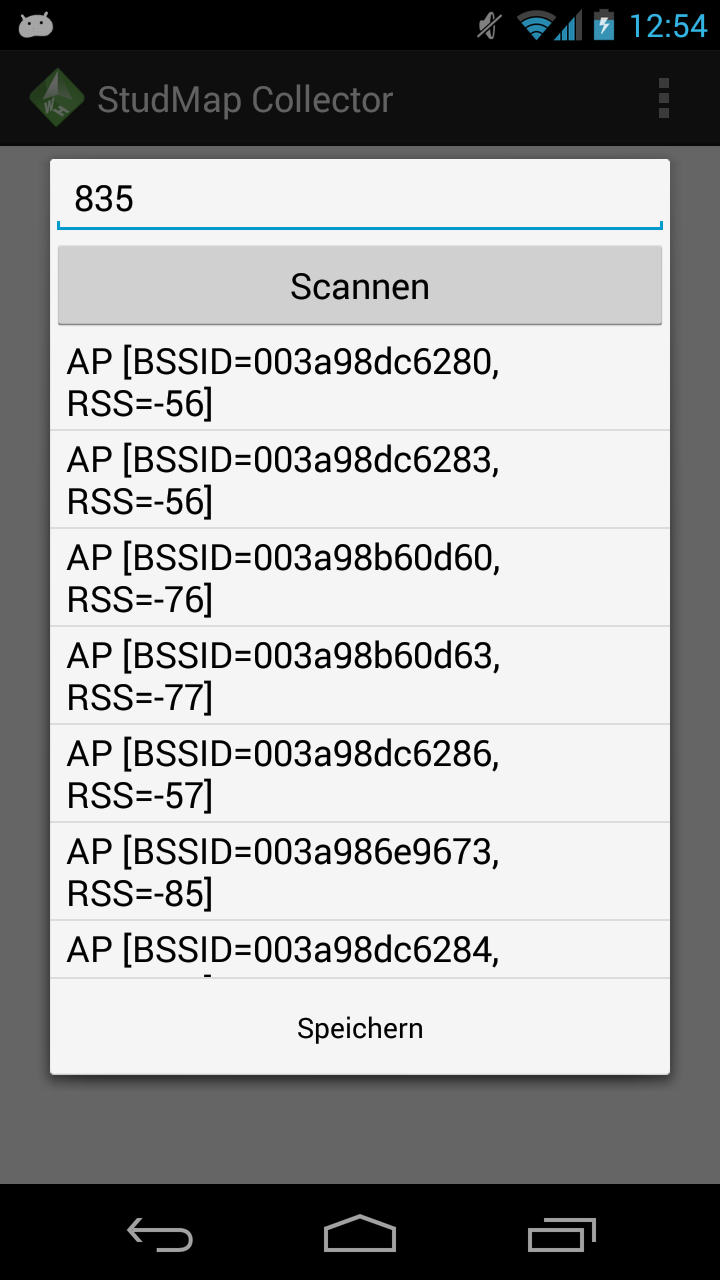
\includegraphics[width=0.5\linewidth]{../Bilder/Collector/WifiScannedScreen}
\label{fig:WifiScannedScreen}
\end{figure}

\chapter{Webservice}
F�r den Zugriff auf die Daten stellen wir den Webservice \texttt{StudMap.Service} zur Verf�gung.
Der Webservice besteht dabei aus zwei Schnittstellen in Form von sogenannten Controller Klassen, die jeweils von der Klasse \texttt{ApiController} \todo{Kurze Beschreibung von ApiController und Controller Klassen im Allgemeinen} abgeleitet sind:
\begin{itemize}
\item \texttt{MapsController}: Verwaltung von Karten- und Routeninformationen
\item \texttt{UsersController}: Verwaltung von Benutzerinformationen
\end{itemize}

Bevor nun die Funktionen der jeweiligen Controller Klasse erl�utert werden, folgt eine �bersicht, �ber die verschiedenen R�ckgabe Werte und ihre Bedeutung.

\section{R�ckgabewerte}
\todo{Erkl�rung der verschiedenen Response Objekte und deren Serialisierung in JSON}

\section{MapsController}
\todo{MapsController dokumentieren}

\section{UsersController}
\label{Webservice_UsersController}

Der \texttt{UsersController} stellt klassische Funktionen zur Benutzerverwaltung zur Verf�gung.

\begin{itemize}
\item Register
\item Login
\item Logout
\item GetActiveUsers
\end{itemize}


\subsection{Register}
Registriert einen neuen Anwender in der Benutzerrolle \textit{Benutzer}.

Aufruf �ber HTTP Post:\\
\url{http://localhost:1129/api/Users/Register?userName=test&password=geheim}

\todo{Verweis auf entsprechenden R�ckgabewert}
\subsection{Login}
Meldet einen bereits registrierten Anwender am System an.

Aufruf �ber HTTP Post:\\
\url{http://localhost:1129/api/Users/Login?userName=test&password=geheim}

\todo{Verweis auf entsprechenden R�ckgabewert}
\subsection{Logout}
Meldet einen angemeldeten Anwender vom System ab.

Aufruf �ber HTTP Get:\\
\url{http://localhost:1129/api/Users/Logout?userName=test}

\todo{Verweis auf entsprechenden R�ckgabewert}
\subsection{GetActiveUsers}
Ermittelt eine Liste der aktuell am System angemeldeten Anwender.

Aufruf �ber HTTP Get:\\
\url{http://localhost:1129/api/Users/GetActiveUsers}

\todo{Verweis auf entsprechenden R�ckgabewert}
\chapter{Verwendung des Webservices}
\todo{Chris Best Practices "Programmier-Handbuch" f�r MapsController schreiben.}

\section{Verwendung der Benutzerschnittstelle}
\label{Verwendung_Benutzerschnittstelle}
\subsection{Registrierung}
Bevor sich ein Benutzer am StudMap System anmelden kann, muss er sich zun�chst �ber die Funktion \nameref{service:Register} registrieren.

\subsection{Aktive und inaktive Benutzer}
Im StudMap System wird zwischen aktiven und inaktiven Benutzern unterschieden. Nachdem sich ein Benutzer am System registriert hat gilt dieser als inaktiv. �ber die Funktion \nameref{service:Login} kann er sich am System anmelden und gilt somit als aktiv.

Damit der angemeldete Benutzer auch aktiv bleibt, sollte sich dieser in einem Zeitintervall von f�nf Minuten �ber die Methode \nameref{service:Login} am System aktiv melden. Nach einer Inaktivit�t von 15 Minuten wird der Benutzer automatisch inaktiv.

�ber die Funktion \nameref{service:Logout} kann sich ein Benutzer wieder vom System abmelden und wird somit inaktiv.

\subsection{Aktive Benutzer abfragen}
Die aktiven Benutzer k�nnen �ber die Funktion \nameref{service:GetActiveUsers} abgefragt werden. Damit die Anzeige der aktiven Benutzer im Client m�glichst aktuell ist, sollte diese Abfrage ebenfalls in regelm��igen Zeitabst�nden erfolgen.
\newpage
\section{Admin}
\label{Admin-Doku}
\subsection{Registrieren}
\begin{enumerate}
\item Aufruf der Webseite: \href{http://193.175.199.115/StudMapAdmin/Account/Register}{http://193.175.199.115/StudMapAdmin/Account/Register}.
		\begin{figure}[H]
		\centering
		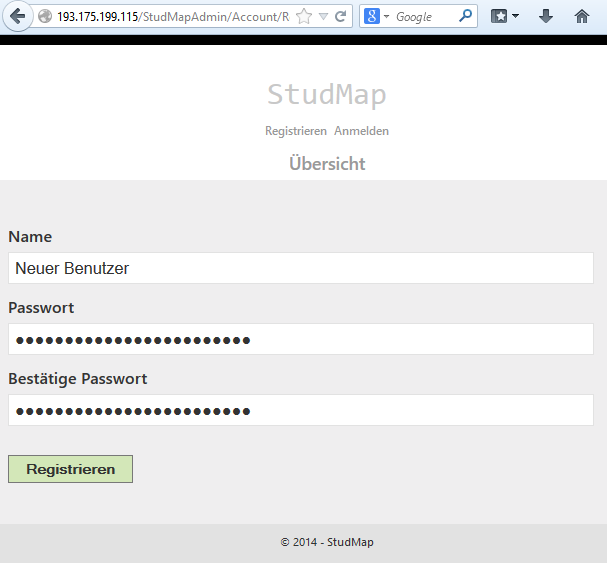
\includegraphics[width=0.7\linewidth]{../Bilder/Admin/AnleitungRegistratur1}
		\label{fig:AnleitungRegistratur1}
		\end{figure}
\item Button \textit{Registrieren} bet�tigen.
\item Datenbankadministrator muss den \nameref{Administrator Rechte versehen}.
\end{enumerate}

\subsection{LogIn / LogOut}
\begin{enumerate}
\item Aufruf der Webseite: \href{http://193.175.199.115/StudMapAdmin/Account/Login}{http://193.175.199.115/StudMapAdmin/Account/Login}.
\item Benutzername und Passwort eingeben.
\item Button \textit{Anmelden} bet�tigen.
\item Sie k�nnen sich jederzeit �ber den Button \textit{Abmelden} ausloggen.
\end{enumerate}

\subsection{Passwort �ndern}
\begin{enumerate}
\item Aufruf der Webseite: \href{http://193.175.199.115/StudMapAdmin/Account/Manage}{http://193.175.199.115/StudMapAdmin/Account/Manage} oder auf eigenen Benutzernamen klicken.
\item Aktuelles Kennwort und gew�nschtes neues Kennwort eingeben. Dieses zus�tzlich best�tigen.
\item Button \textit{Passwort �ndern} bet�tigen.
\end{enumerate}

\subsection{Neue Map anlegen}
\begin{enumerate}
\item Aufruf der Webseite: \href{http://193.175.199.115/StudMapAdmin/Admin/CreateMap}{http://193.175.199.115/StudMapAdmin/Admin/CreateMap} oder auf der Admin Seite auf \textit{Anlegen} klicken.
\item Anschlie�end Map-Namen eingeben und best�tigen.
\item Map kann �ber das Papierkorb-Symbol gel�scht werden.
\end{enumerate}

\subsection{Neuen Floor anlegen}
\begin{enumerate}
\item Aufruf der Webseite: \href{http://193.175.199.115/StudMapAdmin/Admin}{http://193.175.199.115/StudMapAdmin/Admin}. 
\item Anschlie�end auf den Map-Namen klicken.
\item �ber den Button \textit{Anlegen} gelangen Sie nun zur Seite auf der Sie einen Floor hinzuf�gen k�nnen.
\item Den Eintrag MapId wird automatisch �bernommen.
\item Sie geben den Floor-Namen ein und erg�nzen einen Link zu Ihrer Kartengrundlage \footnote{Bevorzugtes Format der Karte sind PDF und PNG Files.}.
\item Abschlie�end bet�tigen Sie den Button \textit{Anlegen}.
\end{enumerate}

\subsection{Men�handhabung des Layers}
\begin{enumerate}
\item Aufruf der Webseite: \href{http://193.175.199.115/StudMapAdmin/Admin}{http://193.175.199.115/StudMapAdmin/Admin}. 
\item Anschlie�end auf den Map-Namen klicken.
\item Dann auf den Floor-Namen klicken.
\item Sie k�nnen �ber das Mausrad in die Karte bzw. aus der Karte hinaus zoomen und das Kartenwerk verschieben, indem Sie die linke Maustaste gedr�ckt halten und die Maus hin und her bewegen.
\item Des Weiteren k�nnen Sie folgende Aktionen ausf�hren, um die Karte mit Meta-Informationen zu erg�nzen:
	\begin{itemize}
	\item \nameref{Knoten anlegen}
	\item \nameref{Kanten anlegen}
	\item \nameref{Knoten loeschen}
	\item \nameref{Knoteninformationen hinterlegen}
	\item \nameref{Knoten mit Knoten auf anderem Floor verbinden}
	\end{itemize} 
\end{enumerate}

\subsubsection*{Knoten anlegen}
\label{Knoten anlegen}
\begin{enumerate}
\item Sie befinden sich auf der Layer-Webseite und haben das Kartenwerk vor Augen.
\item Sie zoomen an die entsprechende Stelle an der Sie einen Knoten erzeugen m�chten mit dem Mausrad.
\item Dann bet�tigen Sie in Kombination mit der \textit{Strg-Taste} die \textit{linke Maustaste}.
\item Abschlie�end m�ssen Sie den Button \textit{Speichern} bet�tigen, den Sie sehen m�ssten wenn sie komplett raus gezoomt haben.
\end{enumerate}

\subsubsection*{Kanten anlegen}
\label{Kanten anlegen}
\begin{enumerate}
\item Sie befinden sich auf der Layer-Webseite und haben das Kartenwerk vor Augen.
\item Zwei Knoten werden miteinander verbunden, indem Sie zuerst einen der beiden Knoten mit einem einfachen Klick mit der \textit{linken Maustaste} markieren.
\item Anschlie�end navigieren Sie zum zweiten Knoten. Durch einen Klick mit der \textit{linken Maustaste} werden beide Knoten mit einer Kante miteinander verbunden.
\item Speichern Sie Ihr Ergebnis �ber den entsprechenden Button ab.
\end{enumerate}

\subsubsection*{Knoten l"oschen}
\label{Knoten loeschen}
\begin{enumerate}
\item Sie befinden sich auf der Layer Webseite und haben das Kartenwerk vor Augen.
\item Sie zoomen zu den Knoten, den es zu entfernen gilt.
\item Markieren Sie den Knoten mit der \textit{linken Maustaste}.
\item Bet�tigen Sie die Taste \textit{Entf} auf Ihrer Tastatur. Der Knoten und anliegende Kanten sind entfernt worden.
\item Vergessen Sie nicht den aktuell vorliegenden Graphen zu speichern.
\end{enumerate}

\subsubsection*{Knoteninformationen hinterlegen}
\label{Knoteninformationen hinterlegen}
\begin{enumerate}
\item Sie befinden sich auf der Layer Webseite und haben das Kartenwerk vor Augen.
\item Durch einen einfachen Klick mit der \textit{rechten Maustaste} erhalten Sie detailliertere Informationen zum Knoten.
		\begin{figure}[H]
		\centering
		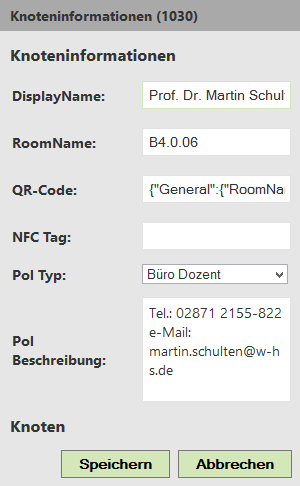
\includegraphics[width=0.3\linewidth]{../Bilder/Admin/AnleitungKnoteninformationen1}
		\label{fig:AnleitungKnoteninformationen1}
		\end{figure}
\item Sie k�nnen die Knoten um Informationen erweitern, indem Sie entsprechende Vermerke in den Textboxen vornehmen.
	\begin{itemize}
	\item Display Name: Sprechender Name des Raumes
	\item RoomName: Einmalige Raumbezeichnung
	\item QR-Code: Von uns automatisierter QR-Code f�r diesen Raum
	\item NFC-Tag: NFC-Tag ID f�r diesen Raum
	\item PoI-Typ: Art des Raumes, z.B. Labor
	\item PoI-Beschreibung: Informationen die diesen Raum genauer beschreiben oder die Sie diesem Knoten zus�tzlich hinterlegen wollen.
	\end{itemize}
\item Die Knoten-ID und die genauen Koordinaten des Knotens, in Prozent, werden angezeigt, nachdem Sie auf das Stichwort \textit{Knoten} mit der Maus navigieren.
\item Info: Erg�nzen Sie einen Knoten um Informationen erst, nachdem Sie den Graphen gespeichert haben. Ansonsten gehen Ihre Eingaben verloren.
\end{enumerate}

\subsubsection*{Knoten stockwerk�bergreifend verbinden}
\label{Knoten mit Knoten auf anderem Floor verbinden}
\begin{enumerate}
\item Sie befinden sich auf der Layer-Webseite und haben das Kartenwerk vor Augen.
\item Zuerst ben�tigen Sie die Knoten-IDs, mit denen Sie Ihren Knoten verbinden m�chten. Also m�ssen Sie sich m�glicherweise die ID eines Knotens auf einem anderen Stockwerk notieren.
\item Bet�tigen Sie die \textit{Shift-Taste} + \textit{Linke Maustaste} auf den Knoten:
		\begin{figure}[H]
		\centering
		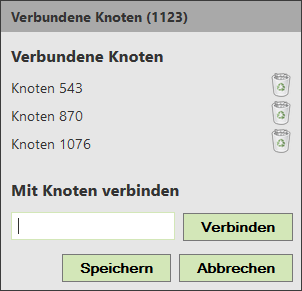
\includegraphics[width=0.3\linewidth]{../Bilder/Admin/AnleitungKnotenMiteinanderVerbinden}
		\label{fig:AnleitungKnotenMiteinanderVerbinden}
		\end{figure}
\item Tragen Sie die ID ein.
\item Dr�cken Sie den Button \textit{Verbinden}.
\item Abschlie�end bet�tigen Sie den Button \textit{Speichern} und zwei Knoten wurden �ber diesen Weg miteinander verbunden.
\end{enumerate}

%Bedienungsanleitung Client
%javascript Schnittstelle

%End-Struktur (Anhang, Quellenverzeichnis, Bib)

\bibliography{Bibliographie}
\bibliographystyle{natdin}
\end{document}